\documentclass[11pt]{article}

% Lecture notes template
\usepackage[margin=1in]{geometry}
\usepackage[T1]{fontenc}
\usepackage{lmodern}
\usepackage{amsmath,amssymb,amsthm}
\usepackage{graphicx}
\usepackage{enumitem}
\usepackage{hyperref}
\usepackage{xcolor}
\usepackage{tikz}
\usetikzlibrary{arrows.meta}
\usepackage{listings}

% Python code in the programming exercises.
\lstset{
    language=Python,
    basicstyle=\ttfamily\small,
    keywordstyle=\color{blue!70!black},
    commentstyle=\color{gray!70!black}\itshape,
    stringstyle=\color{orange!70!black},
    showstringspaces=false,
    upquote=true,
    columns=fullflexible,
    keepspaces=true,
    frame=single,
    rulecolor=\color{gray!40},
    backgroundcolor=\color{gray!6},
    xleftmargin=0.5em,
    xrightmargin=0.5em,
}
% Inline Python code, e.g. \py{np.linalg.solve(A, b)}; unlike \lstinline, it can break at spaces.
\newcommand{\py}[1]{\texttt{\detokenize{#1}}}

% One panel of the gallery of linear transformations of the plane:
% #1, #2 = coordinates of T(e_1); #3, #4 = coordinates of T(e_2); #5 = label.
% The image is drawn by changing TikZ's unit vectors to T(e_1) and T(e_2),
% so a point (x, y) is drawn at x T(e_1) + y T(e_2) = T(x, y).
\newcommand{\gallerypanel}[5]{%
    \begin{tikzpicture}[x=1cm, y=1cm, >=Stealth, baseline=(current bounding box.north)]
        \draw[->, gray] (-1.4,0) -- (2.4,0) node[right] {\small $x$};
        \draw[->, gray] (0,-1.3) -- (0,1.4) node[above] {\small $y$};
        \draw[gray, dashed] (0,0) -- (1,0) -- (1,1) -- (0,1) -- cycle;
        \fill[gray!30] (0.2,0.1) -- (0.4,0.1) -- (0.4,0.45) -- (0.65,0.45) -- (0.65,0.6) -- (0.4,0.6) -- (0.4,0.75) -- (0.8,0.75) -- (0.8,0.9) -- (0.2,0.9) -- cycle;
        \begin{scope}[x={(#1cm,#2cm)}, y={(#3cm,#4cm)}]
            \fill[blue!12] (0,0) -- (1,0) -- (1,1) -- (0,1) -- cycle;
            \draw[blue!70!black, thick] (0,0) -- (1,0) -- (1,1) -- (0,1) -- cycle;
            \fill[orange!85!black] (0.2,0.1) -- (0.4,0.1) -- (0.4,0.45) -- (0.65,0.45) -- (0.65,0.6) -- (0.4,0.6) -- (0.4,0.75) -- (0.8,0.75) -- (0.8,0.9) -- (0.2,0.9) -- cycle;
            \draw[->, very thick, red!80!black] (0,0) -- (1,0);
            \draw[->, very thick, green!50!black] (0,0) -- (0,1);
        \end{scope}
        \node[below, align=center, font=\small] at (0.5,-1.4) {#5};
    \end{tikzpicture}%
}

\title{Lecture 1: Vector Spaces and Linear Transformations}
\author{Linear Algebra}
\date{\today}

\theoremstyle{definition}
\newtheorem{definition}{Definition}[section]
\newtheorem{example}[definition]{Example}
\newtheorem{exercise}[definition]{Exercise}
\theoremstyle{plain}
\newtheorem{theorem}[definition]{Theorem}
\newtheorem{proposition}[definition]{Proposition}
\newtheorem{lemma}[definition]{Lemma}
\newtheorem{corollary}[definition]{Corollary}
\theoremstyle{remark}
\newtheorem{remark}[definition]{Remark}

\DeclareMathOperator{\im}{im}
\DeclareMathOperator{\rank}{rank}
\DeclareMathOperator{\Null}{null}
\DeclareMathOperator{\col}{col}
\DeclareMathOperator{\row}{row}
\DeclareMathOperator{\Span}{span}
\DeclareMathOperator{\RREF}{RREF}
\DeclareMathOperator{\tr}{tr}
\DeclareMathOperator{\diag}{diag}

\begin{document}

\maketitle
\tableofcontents

\section{Number Sets and Fields}

\begin{remark}
    When we want to say that a number $x$ is in a set $S$, we write $x \in S$. When we want to say that a number $x$ is not in a set $S$, we write $x \notin S$.
\end{remark}

\begin{definition}[Number sets]
    $\mathbb{Z}$ is the set of all integers.
    Meaning, \[\mathbb{Z} = \{ \ldots, -2, -1, 0, 1, 2, \ldots \}.\]

    $\mathbb{Q}$ is the set of all rational numbers.
    Meaning, \[\mathbb{Q} = \left\{ \frac{p}{q} : p, q \in \mathbb{Z}, q \neq 0 \right\}.\]

    $\mathbb{R}$ is the set of all real numbers.
    Meaning, $\mathbb{R}$ is obtained from $\mathbb{Q}$ by ``filling in the gaps'': $\mathbb{R} \supset \mathbb{Q}$, every Cauchy sequence in $\mathbb{Q}$ has a limit in $\mathbb{R}$ (completeness), and every real number is the limit of some Cauchy sequence in $\mathbb{Q}$. In other words, $\mathbb{R}$ is the completion of $\mathbb{Q}$.

    $\mathbb{C}$ is the set of all complex numbers.
    Meaning, \[\mathbb{C} = \{ a + bi : a, b \in \mathbb{R} \},\] where $i$ is a number satisfying $i^2 = -1$.
\end{definition}

\begin{example}[Number sets]

    $2$ is a real number, and also an integer and a rational number.

    $\sqrt{2}$ is a real number, but not a rational number.

    $\pi$ is a real number, but not a rational number.

    $e$ is a real number, but not a rational number.

    $2 + 5i$ is a complex number, but not a real number.
\end{example}

\begin{definition}[Field]
    A field is a triple $(\mathbb{F}, +, \cdot)$, where $\mathbb{F}$ is a set and $+$, $\cdot$ are binary operations on $\mathbb{F}$ such that
    \begin{enumerate}
        \item Both $+$ and $\cdot$ are associative, meaning that for all $a, b, c \in \mathbb{F}$,
            \[(a + b) + c = a + (b + c), \qquad (a\cdot b)\cdot c = a\cdot (b\cdot c);\]
        \item Both $+$ and $\cdot$ are commutative, meaning that for all $a, b \in \mathbb{F}$,
            \[a + b = b + a, \qquad a\cdot b = b\cdot a;\]
        \item There exists an additive identity $0 \in \mathbb{F}$ such that $a + 0 = a$ for all $a \in \mathbb{F}$, and there exists a multiplicative identity $1 \in \mathbb{F}$ such that $a\cdot 1 = a$ for all $a \in \mathbb{F}$. Moreover, $0 \neq 1$;
        \item For every $a \in \mathbb{F}$, there exists an additive inverse $-a \in \mathbb{F}$ such that $a + (-a) = 0$, and for every $a \in \mathbb{F}$ with $a \neq 0$, there exists a multiplicative inverse $a^{-1} \in \mathbb{F}$ such that $a\cdot a^{-1} = 1$;
        \item The distributive property holds, meaning $a\cdot (b + c) = a\cdot b + a\cdot c$ for all $a, b, c \in \mathbb{F}$.
    \end{enumerate}
    Saying that $+$ and $\cdot$ are binary operations on $\mathbb{F}$ means that $a + b \in \mathbb{F}$ and $a\cdot b \in \mathbb{F}$ for all $a, b \in \mathbb{F}$; in other words, $\mathbb{F}$ is closed under $+$ and $\cdot$.
\end{definition}

\begin{example}
    The set of real numbers $\mathbb{R}$ with the usual addition and multiplication operations forms a field.
\end{example}

\begin{proof}
    The sum and the product of two real numbers are again real numbers, so $+$ and $\cdot$ are binary operations on $\mathbb{R}$. We need to verify that $\mathbb{R}$ satisfies all the field axioms:
    \begin{enumerate}
        \item Associativity: For any $a, b, c \in \mathbb{R}$, we have $(a + b) + c = a + (b + c)$ and $(a\cdot b)\cdot c = a\cdot (b\cdot c)$.
        \item Commutativity: For any $a, b \in \mathbb{R}$, we have $a + b = b + a$ and $a\cdot b = b\cdot a$.
        \item Identities: The number $0$ is the additive identity since $a + 0 = a$ for all $a \in \mathbb{R}$, and the number $1$ is the multiplicative identity since $a\cdot 1 = a$ for all $a \in \mathbb{R}$. Clearly, $0 \neq 1$.
        \item Inverses: For every $a \in \mathbb{R}$, the additive inverse is $-a$, satisfying $a + (-a) = 0$. For every non-zero $a \in \mathbb{R}$, the multiplicative inverse is $\frac{1}{a}$, satisfying $a\cdot \frac{1}{a} = 1$.
        \item Distributive property: For any $a, b, c \in \mathbb{R}$, we have $a\cdot (b + c) = a\cdot b + a\cdot c$.
    \end{enumerate}
    Since all axioms are satisfied, $\mathbb{R}$ is indeed a field.
\end{proof}

\begin{example}
    The set of integers $\mathbb{Z}$ with the usual addition and multiplication operations does not form a field, since not every non-zero integer has a multiplicative inverse in $\mathbb{Z}$.
    For example, the integer $2$ does not have a multiplicative inverse in $\mathbb{Z}$: there is no integer $b$ with $2 \cdot b = 1$, because the only solution of this equation, $b = \frac{1}{2}$, is not an integer.
\end{example}

\begin{exercise}
    Verify that the set of complex numbers $\mathbb{C}$ and the set of rational numbers $\mathbb{Q}$ with the usual addition and multiplication operations form fields.
\end{exercise}

\section{Vector Spaces}

\begin{definition}[Vector space]
    A vector space over a field $\mathbb{F}$ is a set $V$, whose elements are called vectors, together with two operations:
    \begin{itemize}
        \item vector addition, which assigns to any two vectors $u, v \in V$ a vector $u + v \in V$;
        \item scalar multiplication, which assigns to any scalar $a \in \mathbb{F}$ and any vector $v \in V$ a vector $a \cdot v \in V$,
    \end{itemize}
    satisfying the following axioms:
    \begin{enumerate}
        \item Vector addition is associative and commutative, meaning $(u + v) + w = u + (v + w)$ and $u + v = v + u$ for all $u, v, w \in V$.
        \item There exists an additive identity $0$ in $V$ (called the zero vector, also written $0_V$), meaning $v + 0 = v$ for all $v \in V$.
        \item Every element in $V$ has an additive inverse, meaning for every $v \in V$, there exists $-v \in V$ such that $v + (-v) = 0$.
        \item Scalar multiplication is associative with respect to the field multiplication, meaning $(a \cdot b) \cdot v = a \cdot (b \cdot v)$ for all $a, b \in \mathbb{F}$ and $v \in V$.
        \item Scalar multiplication distributes over vector addition, meaning $a \cdot (u + v) = a \cdot u + a \cdot v$ for all $a \in \mathbb{F}$ and $u, v \in V$.
        \item Scalar multiplication distributes over field addition, meaning $(a + b) \cdot v = a \cdot v + b \cdot v$ for all $a, b \in \mathbb{F}$ and $v \in V$.
        \item The multiplicative identity of the field acts as the identity for scalar multiplication, meaning $1 \cdot v = v$ for all $v \in V$.
    \end{enumerate}
\end{definition}

\begin{example}
    Any field $\mathbb{F}$ is a vector space over itself, with the usual addition and multiplication operations.
\end{example}

\begin{proof}
    Let $V = \mathbb{F}$, and let the vector addition and scalar multiplication be the usual addition and multiplication in the field $\mathbb{F}$. Since $\mathbb{F}$ is closed under $+$ and $\cdot$, both operations give results in $V = \mathbb{F}$. We need to verify that $V$ satisfies all the vector space axioms:
    \begin{enumerate}
        \item Associativity of vector addition: For any $u, v, w \in V$, we have $(u + v) + w = u + (v + w)$, which holds since addition in $\mathbb{F}$ is associative.
        \item Commutativity of vector addition: For any $u, v \in V$, we have $u + v = v + u$, which holds since addition in $\mathbb{F}$ is commutative.
        \item Additive identity: The element $0 \in V$ serves as the additive identity since $v + 0 = v$ for all $v \in V$.
        \item Additive inverse: For every $v \in V$, the additive inverse is $-v$, satisfying $v + (-v) = 0$.
        \item Associativity of scalar multiplication: For any $a, b \in \mathbb{F}$ and $v \in V$, we have $(a \cdot b) \cdot v = a \cdot (b \cdot v)$, which holds since multiplication in $\mathbb{F}$ is associative.
        \item Distributivity of scalar multiplication over vector addition: For any $a \in \mathbb{F}$ and $u, v \in V$, we have $a \cdot (u + v) = a \cdot u + a \cdot v$, which holds since multiplication distributes over addition in $\mathbb{F}$.
        \item Distributivity of scalar multiplication over field addition: For any $a, b \in \mathbb{F}$ and $v \in V$, we have $(a + b) \cdot v = a \cdot v + b \cdot v$, which holds since multiplication distributes over addition in $\mathbb{F}$.
        \item Identity element of scalar multiplication: The multiplicative identity $1$ acts as the identity for scalar multiplication since $1 \cdot v = v$ for all $v \in V$.
    \end{enumerate}
    Since all axioms are satisfied, $V = \mathbb{F}$ is indeed a vector space over itself.
\end{proof}

\begin{corollary}\label{cor:fields}
    $\mathbb{Q}, \mathbb{R},$ and $\mathbb{C}$ are vector spaces over themselves.
\end{corollary}

\begin{definition}[Product of vector spaces]
    Let $V$ and $W$ be vector spaces over the same field $\mathbb{F}$. Their product is the set
    \[V \times W = \{(v, w) : v \in V, \ w \in W\}\]
    of all ordered pairs $(v, w)$ with $v \in V$ and $w \in W$. The operations of vector addition and scalar multiplication are defined component-wise:
    \begin{align*}
        (v_1, w_1) + (v_2, w_2) &= (v_1 + v_2, w_1 + w_2), \\
        a \cdot (v, w) &= (a \cdot v, a \cdot w), \qquad a \in \mathbb{F}.
    \end{align*}
\end{definition}

\begin{proposition}\label{prop:product}
    If $V$ and $W$ are vector spaces over the same field $\mathbb{F}$, then $V \times W$ is also a vector space over $\mathbb{F}$.
\end{proposition}

\begin{proof}
    The operations give results in $V \times W$, since $v_1 + v_2, a \cdot v \in V$ and $w_1 + w_2, a \cdot w \in W$. We need to verify that $V \times W$ satisfies all the vector space axioms. Each of them follows from the corresponding axiom in $V$ and in $W$:
    \begin{enumerate}
        \item Associativity of vector addition: For any $(v_1, w_1), (v_2, w_2), (v_3, w_3) \in V \times W$, we have
        \[
        ((v_1, w_1) + (v_2, w_2)) + (v_3, w_3) = (v_1 + v_2 + v_3, w_1 + w_2 + w_3) = (v_1, w_1) + ((v_2, w_2) + (v_3, w_3)).
        \]
        \item Commutativity of vector addition: For any $(v_1, w_1), (v_2, w_2) \in V \times W$, we have
        \[
        (v_1, w_1) + (v_2, w_2) = (v_1 + v_2, w_1 + w_2) = (v_2 + v_1, w_2 + w_1) = (v_2, w_2) + (v_1, w_1).
        \]
        \item Additive identity: The element $(0_V, 0_W)$ serves as the additive identity since
        \[
        (v, w) + (0_V, 0_W) = (v + 0_V, w + 0_W) = (v, w).
        \]
        \item Additive inverse: For every $(v, w) \in V \times W$, the additive inverse is $(-v, -w)$ satisfying
        \[
        (v, w) + (-v, -w) = (0_V, 0_W).
        \]
        \item Associativity of scalar multiplication: For any $a, b \in \mathbb{F}$ and $(v, w) \in V \times W$, we have
        \[
        a(b(v,w)) = a(b\cdot v, b\cdot w) = (ab\cdot v, ab\cdot w) = (ab)(v,w).
        \]
        \item Distributivity of scalar multiplication over vector addition: For any $a \in \mathbb{F}$ and any $(v_1, w_1)$, $(v_2, w_2) \in V \times W$, we have
        \[
        \begin{aligned}
        a((v_1, w_1) + (v_2, w_2)) &= (a(v_1 + v_2), a(w_1 + w_2)) \\
        &= (a v_1 + a v_2, a w_1 + a w_2) \\
        &= (a v_1, a w_1) + (a v_2, a w_2) \\
        &= a(v_1, w_1) + a(v_2, w_2).
        \end{aligned}
        \]
        \item Distributivity of scalar multiplication over field addition: For any $a, b \in \mathbb{F}$ and $(v, w) \in V \times W$, we have
        \[
        (a + b)(v, w) = ((a + b)v, (a + b)w) = (av + bv, aw + bw) = (av, aw) + (bv, bw) = a(v, w) + b(v, w).
        \]
        \item Identity element of scalar multiplication: For any $(v, w) \in V \times W$, we have
        \[
        1 \cdot (v, w) = (1 \cdot v, 1 \cdot w) = (v, w).
        \]
    \end{enumerate}
    Since all axioms are satisfied, $V \times W$ is a vector space over $\mathbb{F}$.
\end{proof}

\begin{remark}
    For two (or finitely many) vector spaces, the product is also known as the (external) direct sum of the vector spaces, and it is often denoted by $V \oplus W$.
\end{remark}

\begin{definition}[The space $\mathbb{R}^n$]
    Let $n$ be a positive integer. The set $\mathbb{R}^n$ consists of all ordered $n$-tuples of real numbers,
    \[\mathbb{R}^n = \{(x_1, x_2, \ldots, x_n) : x_i \in \mathbb{R} \text{ for } i = 1, 2, \ldots, n\},\]
    and the operations of vector addition and scalar multiplication are defined component-wise:
    \begin{align*}
        (x_1, \ldots, x_n) + (y_1, \ldots, y_n) &= (x_1 + y_1, \ldots, x_n + y_n), \\
        a \cdot (x_1, \ldots, x_n) &= (a x_1, \ldots, a x_n), \qquad a \in \mathbb{R}.
    \end{align*}
\end{definition}

\begin{corollary}
    The set $\mathbb{R}^n$ is a vector space over the field $\mathbb{R}$ for every positive integer $n$.
\end{corollary}

\begin{proof}
    We use induction on $n$. For $n = 1$, $\mathbb{R}^1 = \mathbb{R}$ is a vector space over itself by Corollary~\ref{cor:fields}.

    Now let $n \geq 2$ and assume that $\mathbb{R}^{n-1}$ is a vector space over $\mathbb{R}$. Identify each $n$-tuple $(x_1, \ldots, x_n)$ with the pair $((x_1, \ldots, x_{n-1}), x_n) \in \mathbb{R}^{n-1} \times \mathbb{R}$. Under this identification, the component-wise operations on $\mathbb{R}^n$ are exactly the operations of the product $\mathbb{R}^{n-1} \times \mathbb{R}$. By Proposition~\ref{prop:product}, $\mathbb{R}^{n-1} \times \mathbb{R}$ is a vector space over $\mathbb{R}$, and hence so is $\mathbb{R}^n$.
\end{proof}

\section{Bases and Dimension}

Throughout this section, $V$ is a vector space over a field $\mathbb{F}$.

\begin{definition}[Linear combination and span]
    Let $v_1, v_2, \ldots, v_k \in V$. A linear combination of $v_1, \ldots, v_k$ is a vector of the form
    \[a_1 v_1 + a_2 v_2 + \cdots + a_k v_k, \qquad a_1, \ldots, a_k \in \mathbb{F}.\]
    The span of $v_1, \ldots, v_k$ is the set of all their linear combinations:
    \[\Span\{v_1, \ldots, v_k\} = \{a_1 v_1 + \cdots + a_k v_k : a_1, \ldots, a_k \in \mathbb{F}\}.\]
    We say that $v_1, \ldots, v_k$ span $V$ if $\Span\{v_1, \ldots, v_k\} = V$, i.e., if every vector in $V$ is a linear combination of $v_1, \ldots, v_k$.
\end{definition}

\begin{definition}[Linear independence]
    The vectors $v_1, \ldots, v_k \in V$ are linearly independent if the only way to write the zero vector as a linear combination of them is with all coefficients equal to zero:
    \[a_1 v_1 + a_2 v_2 + \cdots + a_k v_k = 0 \implies a_1 = a_2 = \cdots = a_k = 0.\]
    Otherwise, they are called linearly dependent.

    For an infinite set $S \subseteq V$, we say that $S$ is linearly independent if every finite subset of $S$ is linearly independent, and that $S$ spans $V$ if every vector in $V$ is a linear combination of finitely many vectors from $S$.
\end{definition}

\begin{example}
    In $\mathbb{R}^2$, the vectors $(1, 2)$ and $(2, 4)$ are linearly dependent, since
    \[2 \cdot (1, 2) + (-1) \cdot (2, 4) = (0, 0).\]
    Their span is the line $\Span\{(1, 2), (2, 4)\} = \{(t, 2t) : t \in \mathbb{R}\}$, so they do not span $\mathbb{R}^2$. For example, $(1, 0)$ is not in their span.
\end{example}

\begin{definition}[Basis]
    A basis of a vector space $V$ is a set of vectors in $V$ that is linearly independent and spans $V$.
\end{definition}

\begin{proposition}\label{prop:unique-rep}
    Let $\{v_1, v_2, \ldots, v_n\}$ be a basis of $V$. Then every vector in $V$ can be expressed as a linear combination of the basis vectors in exactly one way.
\end{proposition}

\begin{proof}
    Since the basis spans $V$, every $v \in V$ can be written as $v = a_1 v_1 + \cdots + a_n v_n$ for some $a_1, \ldots, a_n \in \mathbb{F}$. Suppose that also $v = b_1 v_1 + \cdots + b_n v_n$. Subtracting the two expressions gives
    \[(a_1 - b_1) v_1 + \cdots + (a_n - b_n) v_n = 0.\]
    Since $v_1, \ldots, v_n$ are linearly independent, $a_i - b_i = 0$, i.e., $a_i = b_i$ for every $i$. So the two expressions are the same.
\end{proof}

\begin{theorem}
    If a vector space $V$ has a basis consisting of $n$ vectors, then every basis of $V$ consists of exactly $n$ vectors.
\end{theorem}

We state this theorem without proof. It allows us to make the following definition.

\begin{definition}[Dimension]
    A vector space $V$ is said to be finite-dimensional if it has a finite basis. In this case, the dimension of $V$, denoted by $\dim V$, is the number of vectors in any basis of $V$; by the theorem above, this number does not depend on which basis we choose. If a vector space does not have a finite basis, it is called infinite-dimensional.

    By convention, the vector space $\{0\}$ consisting only of the zero vector has dimension $0$ (its basis is the empty set).
\end{definition}

\begin{definition}[Standard basis]
    The standard basis for the vector space $\mathbb{R}^n$ is the set of vectors $\{e_1, e_2, \ldots, e_n\}$, where each $e_i$ is a vector in $\mathbb{R}^n$ with a $1$ in the $i$-th position and $0$s in all other positions. Formally, the standard basis vectors are defined as:
    \[e_i = (0, \ldots, 0, 1, 0, \ldots, 0) \qquad \text{(with $1$ in the $i$-th position)}.\]
\end{definition}

\begin{proposition}
    The standard basis $\{e_1, \ldots, e_n\}$ is a basis of $\mathbb{R}^n$. In particular, $\mathbb{R}^n$ is finite-dimensional and $\dim \mathbb{R}^n = n$.
\end{proposition}

\begin{proof}
    Every vector $x = (x_1, \ldots, x_n) \in \mathbb{R}^n$ can be written as
    \[x = x_1 e_1 + x_2 e_2 + \cdots + x_n e_n,\]
    so the standard basis spans $\mathbb{R}^n$. If $a_1 e_1 + \cdots + a_n e_n = 0$, then $(a_1, \ldots, a_n) = (0, \ldots, 0)$, so $a_1 = \cdots = a_n = 0$. Hence the standard basis is also linearly independent.
\end{proof}

\begin{example}
    Consider the vector space $\mathbb{R}^2$. Its standard basis is the set of vectors $\{(1, 0), (0, 1)\}$. These vectors are linearly independent and span the entire space $\mathbb{R}^2$, meaning that any vector $(x, y) \in \mathbb{R}^2$ can be expressed as a linear combination of these basis vectors:
    \[(x, y) = x \cdot (1, 0) + y \cdot (0, 1).\]
    The dimension of $\mathbb{R}^2$ is $2$, as there are two vectors in the basis.
\end{example}

\begin{example}
    Consider the vector space $\mathbb{R}^3$. Its standard basis is the set of vectors
    \[\{(1, 0, 0), (0, 1, 0), (0, 0, 1)\}.\]
    These vectors are linearly independent and span the entire space $\mathbb{R}^3$, meaning that any vector $(x, y, z) \in \mathbb{R}^3$ can be expressed as a linear combination of these basis vectors:
    \[(x, y, z) = x \cdot (1, 0, 0) + y \cdot (0, 1, 0) + z \cdot (0, 0, 1).\]
    The dimension of $\mathbb{R}^3$ is $3$, as there are three vectors in the basis.
\end{example}

\begin{example}
    The set of all polynomials with real coefficients,
    \[\mathbb{R}[x] = \{a_0 + a_1 x + \cdots + a_d x^d : d \geq 0, \ a_0, \ldots, a_d \in \mathbb{R}\},\]
    is a vector space over $\mathbb{R}$ with the usual addition of polynomials and multiplication of a polynomial by a real number. This vector space is infinite-dimensional.

    You may check for yourself that the set of monomials $\{1, x, x^2, x^3, \ldots\}$ is linearly independent and spans the space of all polynomials, so it is an (infinite) basis of $\mathbb{R}[x]$.

    To see that there is no finite basis, take any finitely many polynomials $p_1, \ldots, p_k \in \mathbb{R}[x]$, and choose an integer $d \geq 0$ such that each $p_i$ has degree at most $d$. Every linear combination of $p_1, \ldots, p_k$ also has degree at most $d$, so $x^{d+1} \notin \Span\{p_1, \ldots, p_k\}$. Hence no finite set of polynomials spans $\mathbb{R}[x]$, and in particular $\mathbb{R}[x]$ has no finite basis.
\end{example}

\section{Linear Transformations}\label{sec:linear}

\begin{definition}[Linear transformation]
    A linear transformation between two vector spaces $V$ and $W$ over the same field $\mathbb{F}$ is a function $T: V \to W$ that satisfies the following two properties for all $u, v \in V$ and all scalars $a \in \mathbb{F}$:
    \begin{enumerate}
        \item Additivity: $T(u + v) = T(u) + T(v)$
        \item Homogeneity: $T(a \cdot v) = a \cdot T(v)$
    \end{enumerate}
\end{definition}

\begin{lemma}\label{lem:zero}
    If $T: V \to W$ is a linear transformation, then $T(0_V) = 0_W$.
\end{lemma}

\begin{proof}
    By additivity, $T(0_V) = T(0_V + 0_V) = T(0_V) + T(0_V)$. Adding $-T(0_V)$ to both sides gives $0_W = T(0_V)$.
\end{proof}

\begin{example}
    Let $T: \mathbb{R}^2 \to \mathbb{R}^2$ be defined by $T(x, y) = (2x + 3y, 4x - y)$. We will verify that $T$ is a linear transformation.

    First, we check additivity:
    \begin{align*}
        T((x_1, y_1) + (x_2, y_2)) &= T(x_1 + x_2, y_1 + y_2) \\
        &= (2(x_1 + x_2) + 3(y_1 + y_2), 4(x_1 + x_2) - (y_1 + y_2)) \\
        &= (2x_1 + 3y_1 + 2x_2 + 3y_2, 4x_1 - y_1 + 4x_2 - y_2) \\
        &= (2x_1 + 3y_1, 4x_1 - y_1) + (2x_2 + 3y_2, 4x_2 - y_2) \\
        &= T(x_1, y_1) + T(x_2, y_2).
    \end{align*}

    Next, we check homogeneity:
    \begin{align*}
        T(a \cdot (x, y)) &= T(ax, ay) \\
        &= (2(ax) + 3(ay), 4(ax) - (ay)) \\
        &= a(2x + 3y, 4x - y) \\
        &= a \cdot T(x, y).
    \end{align*}

    Since both properties hold, $T$ is indeed a linear transformation.
\end{example}

\begin{remark}[Visualizing linear transformations of the plane]
    Every vector of $\mathbb{R}^2$ can be written as $(x, y) = x e_1 + y e_2$, so for a linear transformation $T: \mathbb{R}^2 \to \mathbb{R}^2$,
    \[T(x, y) = x\,T(e_1) + y\,T(e_2).\]
    Hence $T$ is completely determined by the two vectors $T(e_1)$ and $T(e_2)$. In particular, $T$ maps the unit square $\{x e_1 + y e_2 : 0 \leq x, y \leq 1\}$ to the parallelogram $\{x T(e_1) + y T(e_2) : 0 \leq x, y \leq 1\}$ spanned by $T(e_1)$ and $T(e_2)$. The origin stays where it is (Lemma~\ref{lem:zero}), and a grid of equally spaced parallel lines is mapped to a grid of equally spaced parallel lines (or, if $T(e_1)$ and $T(e_2)$ lie on a common line, squashed onto that line). Figure~\ref{fig:T-grid} shows this for the linear transformation of the previous example, for which $T(e_1) = (2, 4)$ and $T(e_2) = (3, -1)$. Figure~\ref{fig:gallery} shows four basic examples; you may check that each of them is linear.
\end{remark}

\begin{figure}[ht]
    \centering
    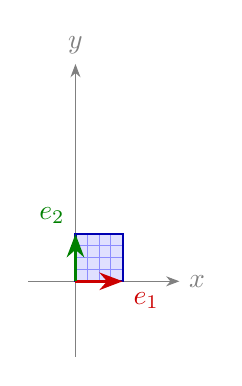
\begin{tikzpicture}[x=0.6cm, y=0.6cm, >=Stealth, baseline=(current bounding box.center)]
        \draw[->, gray] (-1,0) -- (2.2,0) node[right] {$x$};
        \draw[->, gray] (0,-1.6) -- (0,4.6) node[above] {$y$};
        \fill[blue!12] (0,0) -- (1,0) -- (1,1) -- (0,1) -- cycle;
        \foreach \t in {0.25, 0.5, 0.75} {
            \draw[blue!45] (\t,0) -- (\t,1);
            \draw[blue!45] (0,\t) -- (1,\t);
        }
        \draw[blue!70!black, thick] (0,0) -- (1,0) -- (1,1) -- (0,1) -- cycle;
        \draw[->, very thick, red!80!black] (0,0) -- (1,0) node[below right] {$e_1$};
        \draw[->, very thick, green!50!black] (0,0) -- (0,1) node[above left] {$e_2$};
    \end{tikzpicture}
    \quad $\xrightarrow{\quad T \quad}$ \quad
    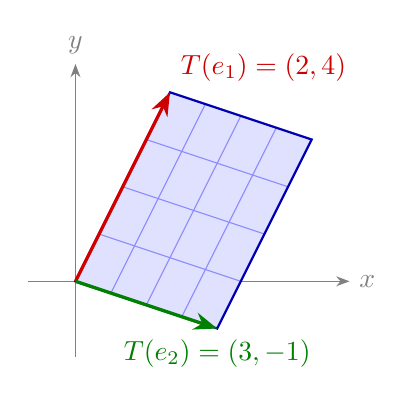
\begin{tikzpicture}[x=0.6cm, y=0.6cm, >=Stealth, baseline=(current bounding box.center)]
        \draw[->, gray] (-1,0) -- (5.8,0) node[right] {$x$};
        \draw[->, gray] (0,-1.6) -- (0,4.6) node[above] {$y$};
        % Unit vectors 0.6 * T(e_1) and 0.6 * T(e_2), so (x, y) is drawn at T(x, y).
        \begin{scope}[x={(1.2cm,2.4cm)}, y={(1.8cm,-0.6cm)}]
            \fill[blue!12] (0,0) -- (1,0) -- (1,1) -- (0,1) -- cycle;
            \foreach \t in {0.25, 0.5, 0.75} {
                \draw[blue!45] (\t,0) -- (\t,1);
                \draw[blue!45] (0,\t) -- (1,\t);
            }
            \draw[blue!70!black, thick] (0,0) -- (1,0) -- (1,1) -- (0,1) -- cycle;
        \end{scope}
        \draw[->, very thick, red!80!black] (0,0) -- (2,4) node[above right] {$T(e_1) = (2, 4)$};
        \draw[->, very thick, green!50!black] (0,0) -- (3,-1) node[below] {$T(e_2) = (3, -1)$};
    \end{tikzpicture}
    \caption[A linear transformation acting on the unit square]{The linear transformation $T(x, y) = (2x + 3y, 4x - y)$ maps the unit square (left) to the parallelogram spanned by $T(e_1)$ and $T(e_2)$ (right). The grid lines inside the square are mapped to equally spaced parallel lines inside the parallelogram.}
    \label{fig:T-grid}
\end{figure}

\begin{figure}[ht]
    \centering
    \gallerypanel{2}{0}{0}{1}{(a) stretch\\ $T(x, y) = (2x, y)$}
    \qquad
    \gallerypanel{0}{1}{-1}{0}{(b) rotation by $90^\circ$\\ $T(x, y) = (-y, x)$}

    \bigskip
    \gallerypanel{1}{0}{0}{-1}{(c) reflection in the $x$-axis\\ $T(x, y) = (x, -y)$}
    \qquad
    \gallerypanel{1}{0}{1}{1}{(d) shear\\ $T(x, y) = (x + y, y)$}
    \caption[Four linear transformations of the plane]{Four linear transformations of the plane. The dashed square and the gray letter F show the unit square before the transformation; the blue parallelogram and the orange letter F show its image. The red and green arrows are $T(e_1)$ and $T(e_2)$. Note that in (c), the image of the letter F is mirrored.}
    \label{fig:gallery}
\end{figure}

\begin{definition}[Kernel]
    The kernel of a linear transformation $T: V \to W$ is the set of all vectors in $V$ that are mapped to the zero vector in $W$. Formally, the kernel is defined as
    \[\ker(T) = \{v \in V : T(v) = 0_W\},\]
    where $0_W$ is the zero vector in $W$.
\end{definition}

\begin{example}\label{ex:ker1}
    Let $T: \mathbb{R}^2 \to \mathbb{R}^2$ be defined by $T(x, y) = (2x + 3y, 4x - y)$. We will find the kernel of $T$.

    To find the kernel, we need to solve the equation $T(x, y) = (0, 0)$:
    \begin{align*}
        2x + 3y &= 0 \\
        4x - y &= 0
    \end{align*}

    From the second equation, we can express $y$ in terms of $x$: $y = 4x$. Substituting this into the first equation gives:
    \begin{align*}
        2x + 3(4x) &= 0 \\
        2x + 12x &= 0 \\
        14x &= 0 \\
        x &= 0
    \end{align*}

    Substituting $x = 0$ back into $y = 4x$, we find that $y = 0$. Therefore, the only solution is $(0, 0)$.

    Thus, the kernel of $T$ is
    \[\ker(T) = \{(0, 0)\}.\]
\end{example}

\begin{example}\label{ex:ker2}
    Let $T: \mathbb{R}^3 \to \mathbb{R}^2$ be defined by $T(x, y, z) = (x + 2y - z, 3x - y + 4z)$. We will find the kernel of $T$.

    To find the kernel, we need to solve the equation $T(x, y, z) = (0, 0)$:
    \begin{align*}
        x + 2y - z &= 0 \\
        3x - y + 4z &= 0
    \end{align*}

    From the first equation, we can express $z$ in terms of $x$ and $y$: $z = x + 2y$. Substituting this into the second equation gives:
    \begin{align*}
        3x - y + 4(x + 2y) &= 0 \\
        3x - y + 4x + 8y &= 0 \\
        7x + 7y &= 0 \\
        x + y &= 0
    \end{align*}

    From this equation, we can express $y$ in terms of $x$: $y = -x$. Substituting this back into the expression for $z$, we get:
    \[z = x + 2(-x) = x - 2x = -x.\]

    Therefore, any vector in the kernel can be expressed as $(x, -x, -x)$ for some scalar $x$. Thus, the kernel of $T$ is
    \[\ker(T) = \{(x, -x, -x) : x \in \mathbb{R}\}.\]
\end{example}

\begin{definition}[Image]
    The image (or range) of a linear transformation $T: V \to W$ is the set of all vectors in $W$ that can be expressed as $T(v)$ for some vector $v \in V$. Formally, the image is defined as
    \[\im(T) = \{w \in W : w = T(v) \text{ for some } v \in V\}.\]
\end{definition}

\begin{example}\label{ex:im1}
    Let $T: \mathbb{R}^2 \to \mathbb{R}^2$ be defined by $T(x, y) = (2x + 3y, 4x - y)$. We will find the image of $T$.

    To find the image, we need to determine all possible outputs of $T$. We will show that every vector of $\mathbb{R}^2$ is an output. Let $(u, v) \in \mathbb{R}^2$ be arbitrary. We look for $x, y \in \mathbb{R}$ such that $T(x, y) = (u, v)$, i.e.,
    \begin{align*}
        u &= 2x + 3y \\
        v &= 4x - y
    \end{align*}

    We can solve this system of equations for $x$ and $y$ in terms of $u$ and $v$. From the second equation, we can express $y$ in terms of $x$ and $v$: $y = 4x - v$. Substituting this into the first equation gives:
    \begin{align*}
        u &= 2x + 3(4x - v) \\
        u &= 2x + 12x - 3v \\
        u &= 14x - 3v
    \end{align*}

    Solving for $x$, we get:
    \[14x = u + 3v \implies x = \frac{u + 3v}{14}.\]

    Substituting this back into the expression for $y$, we get:
    \[y = 4\left(\frac{u + 3v}{14}\right) - v = \frac{4u + 12v - 14v}{14} = \frac{2u - v}{7}.\]

    Let us check that these values work:
    \begin{align*}
        2x + 3y &= \frac{2u + 6v}{14} + \frac{12u - 6v}{14} = u, \\
        4x - y &= \frac{4u + 12v}{14} - \frac{4u - 2v}{14} = v.
    \end{align*}

    Therefore, for any $(u, v) \in \mathbb{R}^2$, we have found $(x, y) \in \mathbb{R}^2$ such that $T(x, y) = (u, v)$. This means that the image of $T$ is all of $\mathbb{R}^2$, i.e.,
    \[\im(T) = \mathbb{R}^2.\]
\end{example}

\begin{example}\label{ex:im2}
    Let $T: \mathbb{R}^3 \to \mathbb{R}^2$ be defined by $T(x, y, z) = (x + 2y - z, 3x - y + 4z)$. We will find the image of $T$.

    As before, we will show that every vector of $\mathbb{R}^2$ is an output of $T$. Let $(u, v) \in \mathbb{R}^2$ be arbitrary. We look for $x, y, z \in \mathbb{R}$ such that $T(x, y, z) = (u, v)$, i.e.,
    \begin{align*}
        u &= x + 2y - z \\
        v &= 3x - y + 4z
    \end{align*}

    From the first equation, we can express $z$ in terms of $x$, $y$, and $u$: $z = x + 2y - u$. Substituting this into the second equation gives:
    \begin{align*}
        v &= 3x - y + 4(x + 2y - u) \\
        v &= 3x - y + 4x + 8y - 4u \\
        v &= 7x + 7y - 4u
    \end{align*}

    Rearranging gives:
    \[7x + 7y = 4u + v.\]

    For any fixed $(u, v)$, this equation describes a line in the $(x, y)$-plane, and every point $(x, y)$ on this line, together with $z = x + 2y - u$, is a solution. For example, we can take $y = 0$ and $x = \frac{4u + v}{7}$, and then $z = x - u = \frac{v - 3u}{7}$. Let us check:
    \[T\left(\frac{4u + v}{7}, 0, \frac{v - 3u}{7}\right) = \left(\frac{(4u + v) - (v - 3u)}{7}, \frac{3(4u + v) + 4(v - 3u)}{7}\right) = (u, v).\]

    Therefore, for any $(u, v) \in \mathbb{R}^2$, we have found $(x, y, z) \in \mathbb{R}^3$ such that $T(x, y, z) = (u, v)$. This means that the image of $T$ is all of $\mathbb{R}^2$, i.e.,
    \[\im(T) = \mathbb{R}^2.\]
\end{example}

\begin{example}\label{ex:kerim-picture}
    Let $T: \mathbb{R}^2 \to \mathbb{R}^2$ be defined by $T(x, y) = (x + 2y, 2x + 4y)$. This map is linear, and it can be written as
    \[T(x, y) = (x + 2y) \cdot (1, 2).\]
    So $T(x, y) = (0, 0)$ if and only if $x + 2y = 0$, and the kernel of $T$ is the line
    \[\ker(T) = \{(-2t, t) : t \in \mathbb{R}\} = \Span\{(-2, 1)\}.\]
    Every output of $T$ is a multiple of $(1, 2)$, and every multiple $s(1, 2) = T(s, 0)$ is an output, so the image of $T$ is the line
    \[\im(T) = \{(s, 2s) : s \in \mathbb{R}\} = \Span\{(1, 2)\}.\]
    More generally, all points of the line $x + 2y = c$, which is parallel to $\ker(T)$, are mapped to the same point $c\,(1, 2)$. So $T$ squashes the whole plane onto the line $\im(T)$, as shown in Figure~\ref{fig:kernel-image}. In particular, $T$ is neither injective nor surjective.
\end{example}

\begin{figure}[ht]
    \centering
    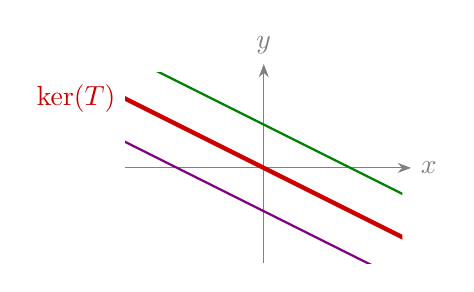
\begin{tikzpicture}[x=0.55cm, y=0.55cm, >=Stealth, baseline=(current bounding box.center)]
        \draw[->, gray] (-3.2,0) -- (3.4,0) node[right] {$x$};
        \draw[->, gray] (0,-2.2) -- (0,2.4) node[above] {$y$};
        \begin{scope}
            \clip (-3.2,-2.2) rectangle (3.2,2.2);
            % The lines x + 2y = c for c = -2, 0, 2, through (c, 0) with direction (-2, 1).
            \draw[thick, violet] (-8,3) -- (4,-3);
            \draw[ultra thick, red!80!black] (-6,3) -- (6,-3);
            \draw[thick, green!50!black] (-4,3) -- (8,-3);
        \end{scope}
        \node[red!80!black, left] at (-3.2,1.6) {$\ker(T)$};
    \end{tikzpicture}
    \quad $\xrightarrow{\quad T \quad}$ \quad
    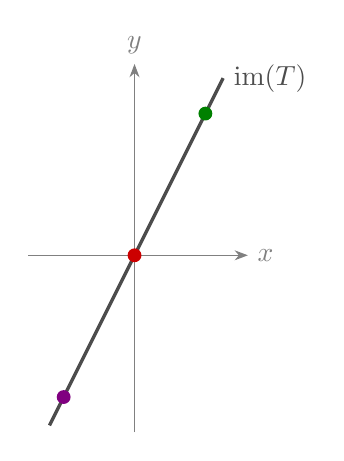
\begin{tikzpicture}[x=0.45cm, y=0.45cm, >=Stealth, baseline=(current bounding box.center)]
        \draw[->, gray] (-3,0) -- (3.2,0) node[right] {$x$};
        \draw[->, gray] (0,-5) -- (0,5.4) node[above] {$y$};
        \draw[very thick, gray!60!black] (-2.4,-4.8) -- (2.5,5) node[right] {$\im(T)$};
        \fill[violet] (-2,-4) circle (2.5pt);
        \fill[red!80!black] (0,0) circle (2.5pt);
        \fill[green!50!black] (2,4) circle (2.5pt);
    \end{tikzpicture}
    \caption[Kernel and image of a linear transformation]{The linear transformation $T(x, y) = (x + 2y, 2x + 4y)$ of Example~\ref{ex:kerim-picture}. Each line $x + 2y = c$ on the left is mapped to the single point $c\,(1, 2)$ on the right, shown in the same color (here $c = -2$, $0$, $2$). The kernel (red, $c = 0$) is mapped to the origin, and the whole plane is squashed onto the line $\im(T)$.}
    \label{fig:kernel-image}
\end{figure}

\subsection{Isomorphisms}

Two vector spaces can look very different and still ``behave in the same way''. For example, a polynomial $a_0 + a_1 x + a_2 x^2$ is added and multiplied by scalars exactly like the list of its coefficients $(a_0, a_1, a_2) \in \mathbb{R}^3$. Isomorphisms make this idea precise.

\begin{definition}[Injective, surjective, bijective]
    A function $f: X \to Y$ between two sets is called
    \begin{itemize}
        \item injective if different inputs give different outputs, i.e., $f(x_1) = f(x_2)$ implies $x_1 = x_2$;
        \item surjective if every element of $Y$ is an output, i.e., for every $y \in Y$ there exists $x \in X$ with $f(x) = y$;
        \item bijective if it is both injective and surjective.
    \end{itemize}
    A function $f$ is bijective if and only if it has an inverse function $f^{-1}: Y \to X$, i.e., a function with $f^{-1}(f(x)) = x$ for all $x \in X$ and $f(f^{-1}(y)) = y$ for all $y \in Y$. Note that a linear transformation $T: V \to W$ is surjective if and only if $\im(T) = W$.
\end{definition}

\begin{definition}[Isomorphism]
    Let $V$ and $W$ be vector spaces over the same field $\mathbb{F}$. An isomorphism from $V$ to $W$ is a bijective linear transformation $T: V \to W$. If there exists an isomorphism from $V$ to $W$, we say that $V$ and $W$ are isomorphic, and we write $V \cong W$.
\end{definition}

\begin{remark}
    An isomorphism $T: V \to W$ matches every vector of $V$ with exactly one vector of $W$, in a way that respects addition and scalar multiplication. So any statement about $V$ that only involves addition and scalar multiplication can be translated into a statement about $W$, and vice versa. In this sense, isomorphic vector spaces are ``the same vector space, written in a different way''.
\end{remark}

To check that a linear transformation is injective, it is enough to look at its kernel.

\begin{lemma}\label{lem:injective}
    A linear transformation $T: V \to W$ is injective if and only if $\ker(T) = \{0_V\}$. Hence $T$ is an isomorphism if and only if $\ker(T) = \{0_V\}$ and $\im(T) = W$.
\end{lemma}

\begin{proof}
    Suppose that $T$ is injective, and let $v \in \ker(T)$. Then $T(v) = 0_W = T(0_V)$ by Lemma~\ref{lem:zero}, so $v = 0_V$.

    Conversely, suppose that $\ker(T) = \{0_V\}$, and let $u, v \in V$ with $T(u) = T(v)$. Using linearity and $(-1) \cdot v = -v$ (Exercise~\ref{ex:axioms}), we get
    \[T(u - v) = T(u + (-1) \cdot v) = T(u) + (-1) \cdot T(v) = T(u) - T(v) = 0_W,\]
    so $u - v \in \ker(T) = \{0_V\}$, i.e., $u = v$.
\end{proof}

\begin{example}\label{ex:iso1}
    The linear transformation $T: \mathbb{R}^2 \to \mathbb{R}^2$, $T(x, y) = (2x + 3y, 4x - y)$, is an isomorphism. Indeed, we found in Example~\ref{ex:ker1} that $\ker(T) = \{(0, 0)\}$, so $T$ is injective by Lemma~\ref{lem:injective}, and we found in Example~\ref{ex:im1} that $\im(T) = \mathbb{R}^2$, so $T$ is surjective. Its inverse is the function we computed in Example~\ref{ex:im1}:
    \[T^{-1}(u, v) = \left(\frac{u + 3v}{14}, \frac{2u - v}{7}\right).\]
\end{example}

\begin{example}
    The linear transformation $T: \mathbb{R}^3 \to \mathbb{R}^2$, $T(x, y, z) = (x + 2y - z, 3x - y + 4z)$, is surjective by Example~\ref{ex:im2}. However, it is not injective, since its kernel is the line $\{(x, -x, -x) : x \in \mathbb{R}\} \neq \{0\}$ (Example~\ref{ex:ker2}). So $T$ is not an isomorphism.

    Similarly, the linear transformation $S: \mathbb{R} \to \mathbb{R}^2$, $S(x) = (x, 0)$, is injective, since $\ker(S) = \{0\}$, but it is not surjective, since $(0, 1)$ is not an output. So $S$ is not an isomorphism either.
\end{example}

\begin{example}\label{ex:iso-poly}
    Let $\mathbb{R}[x]_{\leq 2}$ be the set of polynomials of degree at most $2$, with the usual addition of polynomials and multiplication by real numbers; one can check that it is a vector space over $\mathbb{R}$. The map
    \[T: \mathbb{R}[x]_{\leq 2} \to \mathbb{R}^3, \qquad T(a_0 + a_1 x + a_2 x^2) = (a_0, a_1, a_2),\]
    which lists the coefficients of a polynomial, is an isomorphism. It is linear, since adding two polynomials adds their coefficients, and multiplying a polynomial by a scalar multiplies its coefficients by that scalar. It is injective, since its kernel consists only of the zero polynomial, and it is surjective, since every $(a_0, a_1, a_2) \in \mathbb{R}^3$ is the output $T(a_0 + a_1 x + a_2 x^2)$. Hence $\mathbb{R}[x]_{\leq 2} \cong \mathbb{R}^3$: as far as addition and scalar multiplication are concerned, a polynomial of degree at most $2$ is the same thing as the list of its three coefficients.
\end{example}

\begin{example}
    The complex numbers $\mathbb{C}$ also form a vector space over $\mathbb{R}$, if we only allow multiplication by real scalars. The map $T: \mathbb{C} \to \mathbb{R}^2$, $T(a + bi) = (a, b)$, is linear and bijective (check this!), so it is an isomorphism of vector spaces over $\mathbb{R}$, and $\mathbb{C} \cong \mathbb{R}^2$. This is the familiar picture of complex numbers as points in the plane.
\end{example}

\begin{lemma}\label{lem:composition}
    Let $U$, $V$ and $W$ be vector spaces over the same field $\mathbb{F}$.
    \begin{enumerate}
        \item If $T: U \to V$ and $S: V \to W$ are linear transformations, then their composition $S \circ T: U \to W$, defined by $(S \circ T)(u) = S(T(u))$, is a linear transformation. If $S$ and $T$ are isomorphisms, then so is $S \circ T$.
        \item If $T: V \to W$ is an isomorphism, then its inverse function $T^{-1}: W \to V$ is also linear, and hence an isomorphism.
        \item The identity map $\mathrm{id}_V: V \to V$, $\mathrm{id}_V(v) = v$, is an isomorphism.
    \end{enumerate}
\end{lemma}

\begin{proof}
    (1) For $u_1, u_2, u \in U$ and $a \in \mathbb{F}$, we have
    \begin{align*}
        (S \circ T)(u_1 + u_2) &= S(T(u_1) + T(u_2)) = S(T(u_1)) + S(T(u_2)) = (S \circ T)(u_1) + (S \circ T)(u_2), \\
        (S \circ T)(a u) &= S(a T(u)) = a S(T(u)) = a (S \circ T)(u).
    \end{align*}
    If $S$ and $T$ are bijective, then $S \circ T$ is bijective, with inverse function $T^{-1} \circ S^{-1}$.

    (2) Let $w_1, w_2 \in W$ and $a \in \mathbb{F}$, and let $v_1 = T^{-1}(w_1)$ and $v_2 = T^{-1}(w_2)$. Since $T(v_1 + v_2) = T(v_1) + T(v_2) = w_1 + w_2$, applying $T^{-1}$ gives
    \[T^{-1}(w_1 + w_2) = v_1 + v_2 = T^{-1}(w_1) + T^{-1}(w_2).\]
    Similarly, $T(a v_1) = a T(v_1) = a w_1$ gives $T^{-1}(a w_1) = a v_1 = a T^{-1}(w_1)$. Finally, $T^{-1}$ is bijective, with inverse function $T$.

    (3) The identity map is clearly linear and bijective.
\end{proof}

In particular, $V \cong V$; if $V \cong W$, then $W \cong V$; and if $U \cong V$ and $V \cong W$, then $U \cong W$.

\begin{proposition}\label{prop:iso-basis}
    Let $T: V \to W$ be an isomorphism, and let $\{v_1, \ldots, v_n\}$ be a basis of $V$. Then $\{T(v_1), \ldots, T(v_n)\}$ is a basis of $W$. In particular, if $V$ is finite-dimensional and $V \cong W$, then $W$ is also finite-dimensional and $\dim W = \dim V$.
\end{proposition}

\begin{proof}
    Since $T$ is injective, the vectors $T(v_1), \ldots, T(v_n)$ are $n$ different vectors.

    They span $W$: let $w \in W$. Since $T$ is surjective, $w = T(v)$ for some $v \in V$, and we can write $v = a_1 v_1 + \cdots + a_n v_n$. By linearity, $w = T(v) = a_1 T(v_1) + \cdots + a_n T(v_n)$.

    They are linearly independent: if $a_1 T(v_1) + \cdots + a_n T(v_n) = 0_W$, then by linearity $T(a_1 v_1 + \cdots + a_n v_n) = 0_W$, so $a_1 v_1 + \cdots + a_n v_n \in \ker(T) = \{0_V\}$ by Lemma~\ref{lem:injective}. Since $v_1, \ldots, v_n$ are linearly independent, $a_1 = \cdots = a_n = 0$.
\end{proof}

Conversely, every finite-dimensional vector space is isomorphic to some $\mathbb{R}^n$. To see this, we use coordinates. For the rest of this subsection, we work over the field $\mathbb{R}$; everything works in the same way over any field $\mathbb{F}$, with $\mathbb{F}^n$ in place of $\mathbb{R}^n$.

\begin{definition}[Coordinates]\label{def:coordinates}
    Let $V$ be a vector space over $\mathbb{R}$, and let $\mathcal{B} = (v_1, \ldots, v_n)$ be a basis of $V$ whose vectors are listed in a fixed order (an ordered basis). By Proposition~\ref{prop:unique-rep}, every $v \in V$ can be written in exactly one way as $v = a_1 v_1 + \cdots + a_n v_n$. The vector
    \[[v]_{\mathcal{B}} = (a_1, \ldots, a_n) \in \mathbb{R}^n\]
    is called the coordinate vector of $v$ with respect to $\mathcal{B}$, and the map $\varphi_{\mathcal{B}}: V \to \mathbb{R}^n$, $\varphi_{\mathcal{B}}(v) = [v]_{\mathcal{B}}$, is called the coordinate map.
\end{definition}

\begin{theorem}\label{thm:coordinates}
    Let $V$ be a vector space over $\mathbb{R}$ with an ordered basis $\mathcal{B} = (v_1, \ldots, v_n)$. Then the coordinate map $\varphi_{\mathcal{B}}: V \to \mathbb{R}^n$ is an isomorphism. In particular, every $n$-dimensional vector space over $\mathbb{R}$ is isomorphic to $\mathbb{R}^n$.
\end{theorem}

\begin{proof}
    Let $v = a_1 v_1 + \cdots + a_n v_n$ and $w = b_1 v_1 + \cdots + b_n v_n$, and let $c \in \mathbb{R}$. Then
    \[v + w = (a_1 + b_1) v_1 + \cdots + (a_n + b_n) v_n \qquad \text{and} \qquad cv = (c a_1) v_1 + \cdots + (c a_n) v_n,\]
    and by the uniqueness of these expressions, $[v + w]_{\mathcal{B}} = [v]_{\mathcal{B}} + [w]_{\mathcal{B}}$ and $[cv]_{\mathcal{B}} = c\,[v]_{\mathcal{B}}$. So $\varphi_{\mathcal{B}}$ is linear. It is bijective, because the map $\mathbb{R}^n \to V$, $(a_1, \ldots, a_n) \mapsto a_1 v_1 + \cdots + a_n v_n$, is an inverse function of $\varphi_{\mathcal{B}}$, again by the uniqueness of the expressions.
\end{proof}

\begin{example}
    With the ordered basis $\mathcal{B} = (1, x, x^2)$ of $\mathbb{R}[x]_{\leq 2}$, the coordinate map $\varphi_{\mathcal{B}}$ is exactly the isomorphism of Example~\ref{ex:iso-poly}. With a different ordered basis we get different coordinates: for example, with $\mathcal{B}' = (1, 1 + x, x^2)$, the polynomial $p = 2 + 3x + x^2 = (-1) \cdot 1 + 3 \cdot (1 + x) + 1 \cdot x^2$ has $[p]_{\mathcal{B}'} = (-1, 3, 1)$, while $[p]_{\mathcal{B}} = (2, 3, 1)$.
\end{example}

\begin{corollary}\label{cor:iso-dim}
    Two finite-dimensional vector spaces $V$ and $W$ over $\mathbb{R}$ are isomorphic if and only if $\dim V = \dim W$.
\end{corollary}

\begin{proof}
    If $V \cong W$, then $\dim V = \dim W$ by Proposition~\ref{prop:iso-basis}. Conversely, suppose that $\dim V = \dim W = n$, and choose ordered bases $\mathcal{B}$ of $V$ and $\mathcal{C}$ of $W$. By Theorem~\ref{thm:coordinates} and Lemma~\ref{lem:composition}, the map $\varphi_{\mathcal{C}}^{-1} \circ \varphi_{\mathcal{B}}: V \to W$ is an isomorphism.
\end{proof}

\begin{example}
    Since $\dim \mathbb{R}^2 = 2 \neq 3 = \dim \mathbb{R}^3$, the spaces $\mathbb{R}^2$ and $\mathbb{R}^3$ are not isomorphic: there is no bijective linear transformation between them. On the other hand, any two real vector spaces of dimension $3$, such as $\mathbb{R}[x]_{\leq 2}$ and $\mathbb{R}^3$, are isomorphic. Finally, the infinite-dimensional space $\mathbb{R}[x]$ is not isomorphic to any $\mathbb{R}^n$, by Proposition~\ref{prop:iso-basis}.
\end{example}

\section{Subspaces}

\begin{definition}[Subspace]\label{def:subspace}
    A subspace of a vector space $V$ over $\mathbb{F}$ is a subset $U \subseteq V$ that is itself a vector space under the same operations of vector addition and scalar multiplication defined on $V$. In practice, a subset $U \subseteq V$ is a subspace if and only if it satisfies the following three conditions:
    \begin{enumerate}
        \item The zero vector of $V$ is in $U$, i.e., $0_V \in U$.
        \item $U$ is closed under vector addition: For any $u, v \in U$, we have $u + v \in U$.
        \item $U$ is closed under scalar multiplication: For any $a \in \mathbb{F}$ and any $v \in U$, we have $a \cdot v \in U$.
    \end{enumerate}
\end{definition}

\begin{remark}
    Why are these three conditions enough? Conditions 2 and 3 guarantee that adding vectors of $U$ or multiplying them by scalars never leads outside of $U$. The axioms of associativity, commutativity and distributivity, and $1 \cdot v = v$, then hold in $U$ automatically, because they already hold in $V$. Condition 1 provides the additive identity. Finally, the additive inverse of $v \in U$ is $-v = (-1) \cdot v$ (see Exercise~\ref{ex:axioms} in Section~\ref{sec:exercises}), which lies in $U$ by condition 3.
\end{remark}

\begin{example}
    Let $V = \mathbb{R}^3$ and consider the subset $U = \{(x, y, z) \in \mathbb{R}^3 : x + y + z = 0\}$. We will verify that $U$ is a subspace of $V$.

    First, we check that the zero vector is in $U$:
    \[0_V = (0, 0, 0) \in U \text{ since } 0 + 0 + 0 = 0.\]

    Next, we check closure under vector addition. Let $(x_1, y_1, z_1), (x_2, y_2, z_2) \in U$. Then we have:
    \[x_1 + y_1 + z_1 = 0 \qquad \text{and} \qquad x_2 + y_2 + z_2 = 0.\]
    Now consider their sum:
    \[(x_1, y_1, z_1) + (x_2, y_2, z_2) = (x_1 + x_2, y_1 + y_2, z_1 + z_2).\]
    We need to check if this sum is in $U$:
    \[(x_1 + x_2) + (y_1 + y_2) + (z_1 + z_2) = (x_1 + y_1 + z_1) + (x_2 + y_2 + z_2) = 0 + 0 = 0.\]
    Thus, $(x_1 + x_2, y_1 + y_2, z_1 + z_2) \in U$.

    Finally, we check closure under scalar multiplication. Let $a \in \mathbb{R}$ and $(x, y, z) \in U$. Then we have:
    \[x + y + z = 0.\]
    Now consider the scalar multiple:
    \[a \cdot (x, y, z) = (ax, ay, az).\]
    We need to check if this scalar multiple is in $U$:
    \[ax + ay + az = a(x + y + z) = a \cdot 0 = 0.\]
    Thus, $(ax, ay, az) \in U$.

    Therefore, $U$ is a subspace of $\mathbb{R}^3$.
\end{example}

\begin{theorem}\label{thm:kerim}
    Let $T: V \to W$ be a linear transformation. Then the kernel $\ker(T)$ is a subspace of $V$, and the image $\im(T)$ is a subspace of $W$.
\end{theorem}

\begin{proof}
    \textbf{1. Image is a subspace of $W$:}
    \begin{enumerate}
        \item The zero vector of $W$ is in $\im(T)$ since $T(0_V) = 0_W$ by Lemma~\ref{lem:zero}.
        \item Let $w_1, w_2 \in \im(T)$. Then there exist $v_1, v_2 \in V$ such that $T(v_1) = w_1$ and $T(v_2) = w_2$. We have:
        \[w_1 + w_2 = T(v_1) + T(v_2) = T(v_1 + v_2) \in \im(T).\]
        \item Let $a \in \mathbb{F}$ and $w \in \im(T)$. Then there exists $v \in V$ such that $T(v) = w$. We have:
        \[a \cdot w = a \cdot T(v) = T(a \cdot v) \in \im(T).\]
    \end{enumerate}
    Therefore, $\im(T)$ is a subspace of $W$.

    \textbf{2. Kernel is a subspace of $V$:}
    \begin{enumerate}
        \item The zero vector of $V$ is in $\ker(T)$ since $T(0_V) = 0_W$ by Lemma~\ref{lem:zero}.
        \item Let $v_1, v_2 \in \ker(T)$. Then we have:
        \[T(v_1 + v_2) = T(v_1) + T(v_2) = 0_W + 0_W = 0_W,\]
        which implies that $v_1 + v_2 \in \ker(T)$.
        \item Let $a \in \mathbb{F}$ and $v \in \ker(T)$. Then we have:
        \[T(a \cdot v) = a \cdot T(v) = a \cdot 0_W = 0_W,\]
        which implies that $a \cdot v \in \ker(T)$.
    \end{enumerate}
    Therefore, $\ker(T)$ is a subspace of $V$.
\end{proof}

\section{Matrices}

\begin{definition}[Matrix]
    A matrix is a rectangular array of numbers arranged in rows and columns. An $m \times n$ matrix has $m$ rows and $n$ columns, and is typically denoted by a capital letter, such as $A$. The entry in the $i$-th row and $j$-th column of the matrix $A$ is denoted by $A_{ij}$.
\end{definition}

\begin{example}
    Let $A$ be a $2 \times 3$ matrix given by
    \[A = \begin{pmatrix}
        1 & 2 & 3 \\
        4 & 5 & 6
    \end{pmatrix}.\]
    The entry in the first row and second column is $A_{12} = 2$, and the entry in the second row and third column is $A_{23} = 6$.
\end{example}

\begin{definition}[Transpose]
    The transpose of an $m \times n$ matrix $A$ is the $n \times m$ matrix $A^\top$ with entries $(A^\top)_{ij} = A_{ji}$. In other words, the rows of $A$ become the columns of $A^\top$.
\end{definition}

\begin{example}
    For the matrix $A$ from the previous example,
    \[A^\top = \begin{pmatrix}
        1 & 4 \\
        2 & 5 \\
        3 & 6
    \end{pmatrix}.\]
\end{example}

When working with matrices, we write vectors of $\mathbb{R}^n$ as columns, i.e., as $n \times 1$ matrices. To save space, we often write such a column vector as the transpose of a row:
\[x = (x_1, x_2, \ldots, x_n)^\top = \begin{pmatrix}
    x_1 \\
    x_2 \\
    \vdots \\
    x_n
\end{pmatrix}.\]

\begin{definition}[Matrix--vector product]
    Let $A$ be an $m \times n$ matrix and $x = (x_1, \ldots, x_n)^\top \in \mathbb{R}^n$. The product $Ax$ is the vector in $\mathbb{R}^m$ whose $i$-th entry is
    \[(Ax)_i = A_{i1} x_1 + A_{i2} x_2 + \cdots + A_{in} x_n, \qquad i = 1, \ldots, m.\]
    Note that $Ax$ is only defined when the number of columns of $A$ equals the number of entries of $x$.
\end{definition}

\begin{remark}\label{rem:columns}
    If $a_1, a_2, \ldots, a_n \in \mathbb{R}^m$ denote the columns of $A$, then
    \[Ax = x_1 a_1 + x_2 a_2 + \cdots + x_n a_n,\]
    since the $i$-th entry of the right-hand side is $x_1 A_{i1} + x_2 A_{i2} + \cdots + x_n A_{in}$. In words: $Ax$ is the linear combination of the columns of $A$ whose coefficients are the entries of $x$.
\end{remark}

\begin{example}\label{ex:matvec}
    Let $A = \begin{pmatrix} 1 & 2 & 3 \\ 4 & 5 & 6 \end{pmatrix}$ and $x = (1, 0, -1)^\top$. Then
    \[Ax = \begin{pmatrix}
        1 \cdot 1 + 2 \cdot 0 + 3 \cdot (-1) \\
        4 \cdot 1 + 5 \cdot 0 + 6 \cdot (-1)
    \end{pmatrix} = \begin{pmatrix}
        -2 \\
        -2
    \end{pmatrix} = 1 \cdot \begin{pmatrix} 1 \\ 4 \end{pmatrix} + 0 \cdot \begin{pmatrix} 2 \\ 5 \end{pmatrix} + (-1) \cdot \begin{pmatrix} 3 \\ 6 \end{pmatrix}.\]
\end{example}

\begin{remark}
    For any $m \times n$ matrix $A$, the map $x \mapsto Ax$ is a linear transformation $\mathbb{R}^n \to \mathbb{R}^m$. Indeed, for $x, y \in \mathbb{R}^n$ and $c \in \mathbb{R}$,
    \[(A(x + y))_i = \sum_{j=1}^n A_{ij}(x_j + y_j) = \sum_{j=1}^n A_{ij} x_j + \sum_{j=1}^n A_{ij} y_j = (Ax)_i + (Ay)_i,\]
    and similarly $(A(cx))_i = c\,(Ax)_i$. The next theorem shows that, conversely, every linear transformation $\mathbb{R}^n \to \mathbb{R}^m$ is of this form.
\end{remark}

\begin{theorem}\label{thm:matrix}
    Any linear transformation $T: \mathbb{R}^n \to \mathbb{R}^m$ can be represented by an $m \times n$ matrix $A$ such that for any vector $x \in \mathbb{R}^n$, we have
    \[T(x) = Ax.\]
    The $i$-th column of $A$ is the vector $T(e_i)$.
\end{theorem}

\begin{proof}
    Let $T: \mathbb{R}^n \to \mathbb{R}^m$ be a linear transformation. We will construct an $m \times n$ matrix $A$ that represents $T$.

    Let $\{e_1, e_2, \ldots, e_n\}$ be the standard basis for $\mathbb{R}^n$, where $e_i$ is the vector with a $1$ in the $i$-th position and $0$s elsewhere. For each basis vector $e_i$, we compute $T(e_i)$, which is a vector in $\mathbb{R}^m$. Let
    \[T(e_i) = \begin{pmatrix}
        T(e_i)_1 \\
        T(e_i)_2 \\
        \vdots \\
        T(e_i)_m
    \end{pmatrix}.\]

    We define the matrix $A$ as the matrix whose $i$-th column is $T(e_i)$:
    \[A = \begin{pmatrix}
        T(e_1)_1 & T(e_2)_1 & \cdots & T(e_n)_1 \\
        T(e_1)_2 & T(e_2)_2 & \cdots & T(e_n)_2 \\
        \vdots & \vdots & \ddots & \vdots \\
        T(e_1)_m & T(e_2)_m & \cdots & T(e_n)_m
    \end{pmatrix}.\]

    Now, for any vector $x = (x_1, x_2, \ldots, x_n)^\top \in \mathbb{R}^n$, we can express $x$ as a linear combination of the basis vectors:
    \[x = x_1 e_1 + x_2 e_2 + \cdots + x_n e_n.\]

    Applying the linear transformation $T$ to $x$ and using additivity and homogeneity, we have:
    \[T(x) = T(x_1 e_1 + x_2 e_2 + \cdots + x_n e_n) = x_1 T(e_1) + x_2 T(e_2) + \cdots + x_n T(e_n).\]

    By Remark~\ref{rem:columns}, the right-hand side is exactly the linear combination of the columns of $A$ with coefficients $x_1, \ldots, x_n$, that is,
    \[T(x) = A x.\]
    Therefore, we have shown that any linear transformation $T: \mathbb{R}^n \to \mathbb{R}^m$ can be represented by an $m \times n$ matrix $A$ such that $T(x) = Ax$ for all $x \in \mathbb{R}^n$.
\end{proof}

\begin{example}\label{ex:matT}
    Let $T: \mathbb{R}^2 \to \mathbb{R}^2$ be defined by $T(x, y) = (x - y, 2x + 3y)$. We will find the matrix representation of $T$.

    First, we compute $T(e_1)$ and $T(e_2)$, where $e_1 = (1, 0)$ and $e_2 = (0, 1)$ are the standard basis vectors for $\mathbb{R}^2$:
    \begin{align*}
        T(e_1) &= T(1, 0) = (1 - 0, 2 \cdot 1 + 3 \cdot 0) = (1, 2), \\
        T(e_2) &= T(0, 1) = (0 - 1, 2 \cdot 0 + 3 \cdot 1) = (-1, 3).
    \end{align*}

    Now we can construct the matrix $A$ that represents $T$:
    \[A = \begin{pmatrix}
        T(e_1)_1 & T(e_2)_1 \\
        T(e_1)_2 & T(e_2)_2
    \end{pmatrix} = \begin{pmatrix}
        1 & -1 \\
        2 & 3
    \end{pmatrix}.\]

    Therefore, the matrix representation of the linear transformation $T$ is
    \[A = \begin{pmatrix}
        1 & -1 \\
        2 & 3
    \end{pmatrix}.\]
\end{example}

\begin{example}
    Let $T: \mathbb{R}^3 \to \mathbb{R}^2$ be defined by $T(x, y, z) = (x + 2y - z, 3x - y + 4z)$. We will find the matrix representation of $T$.

    First, we compute $T(e_1)$, $T(e_2)$, and $T(e_3)$, where $e_1 = (1, 0, 0)$, $e_2 = (0, 1, 0)$, and $e_3 = (0, 0, 1)$ are the standard basis vectors for $\mathbb{R}^3$:
    \begin{align*}
        T(e_1) &= T(1, 0, 0) = (1 + 2 \cdot 0 - 0, 3 \cdot 1 - 0 + 4 \cdot 0) = (1, 3), \\
        T(e_2) &= T(0, 1, 0) = (0 + 2 \cdot 1 - 0, 3 \cdot 0 - 1 + 4 \cdot 0) = (2, -1), \\
        T(e_3) &= T(0, 0, 1) = (0 + 2 \cdot 0 - 1, 3 \cdot 0 - 0 + 4 \cdot 1) = (-1, 4).
    \end{align*}

    Now we can construct the matrix $A$ that represents $T$:
    \[A = \begin{pmatrix}
        T(e_1)_1 & T(e_2)_1 & T(e_3)_1 \\
        T(e_1)_2 & T(e_2)_2 & T(e_3)_2
    \end{pmatrix} = \begin{pmatrix}
        1 & 2 & -1 \\
        3 & -1 & 4
    \end{pmatrix}.\]

    Therefore, the matrix representation of the linear transformation $T$ is
    \[A = \begin{pmatrix}
        1 & 2 & -1 \\
        3 & -1 & 4
    \end{pmatrix}.\]
\end{example}

\subsection{Matrix operations}

So far, we have used matrices to represent linear transformations. In this subsection, we learn how to add and multiply matrices; inverses of matrices are discussed in Subsection~\ref{subsec:inverse}, after we have developed row reduction. We write $\mathbb{R}^{m \times n}$ for the set of all $m \times n$ matrices with real entries. For $A \in \mathbb{R}^{m \times n}$, we write $T_A: \mathbb{R}^n \to \mathbb{R}^m$ for the linear transformation $T_A(x) = Ax$.

\subsubsection{Matrix addition}

\begin{definition}[Matrix addition and scalar multiplication]
    Let $A$ and $B$ be $m \times n$ matrices and $c \in \mathbb{R}$. The sum $A + B$ and the scalar multiple $cA$ are the $m \times n$ matrices with entries
    \[(A + B)_{ij} = A_{ij} + B_{ij}, \qquad (cA)_{ij} = c A_{ij}.\]
    In other words, matrices are added and multiplied by scalars entry by entry. The sum $A + B$ is only defined when $A$ and $B$ have the same size.
\end{definition}

\begin{example}
    Let
    \[A = \begin{pmatrix}
        1 & 2 & 3 \\
        4 & 5 & 6
    \end{pmatrix}, \qquad B = \begin{pmatrix}
        0 & -1 & 2 \\
        3 & 1 & -2
    \end{pmatrix}.\]
    Then
    \[A + B = \begin{pmatrix}
        1 + 0 & 2 + (-1) & 3 + 2 \\
        4 + 3 & 5 + 1 & 6 + (-2)
    \end{pmatrix} = \begin{pmatrix}
        1 & 1 & 5 \\
        7 & 6 & 4
    \end{pmatrix},\]
    and
    \[2A = \begin{pmatrix}
        2 & 4 & 6 \\
        8 & 10 & 12
    \end{pmatrix}.\]
    On the other hand, $A + A^\top$ is not defined, since $A$ is a $2 \times 3$ matrix and $A^\top$ is a $3 \times 2$ matrix.
\end{example}

\begin{remark}\label{rem:matrix-space}
    With these operations, $\mathbb{R}^{m \times n}$ is a vector space over $\mathbb{R}$. Indeed, an $m \times n$ matrix is just a list of $mn$ real numbers arranged in a rectangle, and the operations are component-wise, exactly as in $\mathbb{R}^{mn}$. The zero vector of this space is the zero matrix $0$, all of whose entries are $0$, and the additive inverse of $A$ is $-A = (-1)A$. We write $A - B = A + (-B)$. Moreover, $\dim \mathbb{R}^{m \times n} = mn$: a basis consists of the $mn$ matrices that have a single entry equal to $1$ and all other entries equal to $0$.
\end{remark}

\begin{remark}
    Matrix addition corresponds to adding linear transformations: for every $x \in \mathbb{R}^n$,
    \[(A + B)x = Ax + Bx, \qquad (cA)x = c(Ax).\]
    Indeed, $((A + B)x)_i = \sum_j (A_{ij} + B_{ij}) x_j = \sum_j A_{ij} x_j + \sum_j B_{ij} x_j = (Ax)_i + (Bx)_i$, and similarly for $cA$.
\end{remark}

\subsubsection{Matrix multiplication}

Let $A$ be an $m \times n$ matrix and $B$ an $n \times p$ matrix. Then $T_B: \mathbb{R}^p \to \mathbb{R}^n$ and $T_A: \mathbb{R}^n \to \mathbb{R}^m$, so we can first apply $T_B$ and then $T_A$. The result is the composition
\[T_A \circ T_B: \mathbb{R}^p \to \mathbb{R}^m, \qquad x \mapsto A(Bx),\]
which is again a linear transformation by Lemma~\ref{lem:composition}. By Theorem~\ref{thm:matrix}, it is represented by an $m \times p$ matrix, whose $j$-th column is $A(Be_j) = Ab_j$, where $b_j = Be_j$ is the $j$-th column of $B$ (Remark~\ref{rem:columns}). The $i$-th entry of $Ab_j$ is $\sum_{k} A_{ik} B_{kj}$. This motivates the following definition.

\begin{definition}[Matrix multiplication]
    Let $A$ be an $m \times n$ matrix and $B$ an $n \times p$ matrix. The product $AB$ is the $m \times p$ matrix with entries
    \[(AB)_{ij} = A_{i1} B_{1j} + A_{i2} B_{2j} + \cdots + A_{in} B_{nj} = \sum_{k=1}^n A_{ik} B_{kj}.\]
    The product $AB$ is only defined when the number of columns of $A$ equals the number of rows of $B$. An $m \times n$ matrix times an $n \times p$ matrix is an $m \times p$ matrix.
\end{definition}

\begin{remark}\label{rem:two-views}
    There are two useful ways to think about the product $AB$:
    \begin{itemize}
        \item Entry by entry: $(AB)_{ij}$ is obtained by multiplying the entries of the $i$-th row of $A$ with the corresponding entries of the $j$-th column of $B$, and adding up the results.
        \item Column by column: the $j$-th column of $AB$ is $Ab_j$, where $b_j$ is the $j$-th column of $B$:
        \[AB = A \begin{pmatrix} b_1 & b_2 & \cdots & b_p \end{pmatrix} = \begin{pmatrix} Ab_1 & Ab_2 & \cdots & Ab_p \end{pmatrix}.\]
        In particular, if $p = 1$, then $B$ is a single column $x$, and $AB$ is the matrix--vector product $Ax$.
    \end{itemize}
\end{remark}

\begin{example}
    Let
    \[A = \begin{pmatrix}
        1 & 2 & 3 \\
        4 & 5 & 6
    \end{pmatrix}, \qquad B = \begin{pmatrix}
        1 & 0 \\
        0 & 1 \\
        -1 & 2
    \end{pmatrix}.\]
    Since $A$ is $2 \times 3$ and $B$ is $3 \times 2$, the product $AB$ is a $2 \times 2$ matrix. For example, its $(1, 1)$ entry is obtained from the first row of $A$ and the first column of $B$:
    \[(AB)_{11} = 1 \cdot 1 + 2 \cdot 0 + 3 \cdot (-1) = -2.\]
    Computing all four entries in the same way, we get
    \[AB = \begin{pmatrix}
        1 \cdot 1 + 2 \cdot 0 + 3 \cdot (-1) & 1 \cdot 0 + 2 \cdot 1 + 3 \cdot 2 \\
        4 \cdot 1 + 5 \cdot 0 + 6 \cdot (-1) & 4 \cdot 0 + 5 \cdot 1 + 6 \cdot 2
    \end{pmatrix} = \begin{pmatrix}
        -2 & 8 \\
        -2 & 17
    \end{pmatrix}.\]
    Note that the first column of $AB$ is $A(1, 0, -1)^\top = (-2, -2)^\top$, which we computed in Example~\ref{ex:matvec}.

    The product $BA$ is also defined, but it is a $3 \times 3$ matrix:
    \[BA = \begin{pmatrix}
        1 & 2 & 3 \\
        4 & 5 & 6 \\
        7 & 8 & 9
    \end{pmatrix}.\]
    In particular, $AB \neq BA$.
\end{example}

\begin{theorem}\label{thm:composition}
    Let $A$ be an $m \times n$ matrix and $B$ an $n \times p$ matrix. Then for every $x \in \mathbb{R}^p$,
    \[(AB)x = A(Bx).\]
    In other words, $AB$ is the matrix of the composition $T_A \circ T_B$: multiplying matrices corresponds to composing linear transformations.
\end{theorem}

\begin{proof}
    This holds by construction, but we can also check it directly. For each $i = 1, \ldots, m$,
    \begin{align*}
        ((AB)x)_i &= \sum_{j=1}^p (AB)_{ij} x_j = \sum_{j=1}^p \sum_{k=1}^n A_{ik} B_{kj} x_j \\
        &= \sum_{k=1}^n A_{ik} \left(\sum_{j=1}^p B_{kj} x_j\right) = \sum_{k=1}^n A_{ik} (Bx)_k = (A(Bx))_i. \qedhere
    \end{align*}
\end{proof}

\begin{example}
    Let $S, T: \mathbb{R}^2 \to \mathbb{R}^2$ be the linear transformations $S(x, y) = (2x + 3y, 4x - y)$ from Example~\ref{ex:ker1} and $T(x, y) = (x - y, 2x + 3y)$ from Example~\ref{ex:matT}. Their matrices are
    \[A_S = \begin{pmatrix}
        2 & 3 \\
        4 & -1
    \end{pmatrix}, \qquad A_T = \begin{pmatrix}
        1 & -1 \\
        2 & 3
    \end{pmatrix}.\]
    Computing the composition directly, we get
    \begin{align*}
        T(S(x, y)) &= T(2x + 3y, 4x - y) \\
        &= \big((2x + 3y) - (4x - y), \ 2(2x + 3y) + 3(4x - y)\big) \\
        &= (-2x + 4y, 16x + 3y).
    \end{align*}
    On the other hand,
    \[A_T A_S = \begin{pmatrix}
        1 \cdot 2 + (-1) \cdot 4 & 1 \cdot 3 + (-1) \cdot (-1) \\
        2 \cdot 2 + 3 \cdot 4 & 2 \cdot 3 + 3 \cdot (-1)
    \end{pmatrix} = \begin{pmatrix}
        -2 & 4 \\
        16 & 3
    \end{pmatrix},\]
    which is exactly the matrix of $T \circ S$, as Theorem~\ref{thm:composition} predicts.
\end{example}

\begin{definition}[Identity matrix]
    The $n \times n$ identity matrix $I_n$ is the matrix with $1$s on the diagonal and $0$s everywhere else:
    \[(I_n)_{ij} = \begin{cases}
        1 & \text{if } i = j, \\
        0 & \text{if } i \neq j,
    \end{cases} \qquad I_n = \begin{pmatrix}
        1 & 0 & \cdots & 0 \\
        0 & 1 & \cdots & 0 \\
        \vdots & \vdots & \ddots & \vdots \\
        0 & 0 & \cdots & 1
    \end{pmatrix}.\]
    Its columns are the standard basis vectors $e_1, \ldots, e_n$, so $I_n x = x$ for every $x \in \mathbb{R}^n$, i.e., $I_n$ represents the identity map. When the size is clear, we simply write $I$.
\end{definition}

\begin{proposition}\label{prop:mult-props}
    Let $A$, $B$, $C$ be matrices and $c \in \mathbb{R}$. Whenever the sizes are such that the sums and products below are defined, we have:
    \begin{enumerate}
        \item Associativity: $(AB)C = A(BC)$;
        \item Distributivity: $A(B + C) = AB + AC$ and $(A + B)C = AC + BC$;
        \item Scalars: $c(AB) = (cA)B = A(cB)$;
        \item Identity: $I_m A = A = A I_n$ for every $m \times n$ matrix $A$;
        \item Transpose: $(AB)^\top = B^\top A^\top$.
    \end{enumerate}
\end{proposition}

\begin{proof}
    All five properties are checked by comparing entries. For associativity,
    \begin{align*}
        ((AB)C)_{ij} &= \sum_{l} (AB)_{il} C_{lj} = \sum_{l} \sum_{k} A_{ik} B_{kl} C_{lj} \\
        &= \sum_{k} A_{ik} \left(\sum_{l} B_{kl} C_{lj}\right) = \sum_{k} A_{ik} (BC)_{kj} = (A(BC))_{ij}.
    \end{align*}
    For the first distributive law, $(A(B + C))_{ij} = \sum_k A_{ik}(B_{kj} + C_{kj}) = \sum_k A_{ik} B_{kj} + \sum_k A_{ik} C_{kj} = (AB + AC)_{ij}$; the second distributive law and the rule for scalars are checked in the same way. For the identity, $(I_m A)_{ij} = \sum_k (I_m)_{ik} A_{kj} = A_{ij}$, since the only nonzero term is the one with $k = i$; similarly, $A I_n = A$. Finally, for the transpose,
    \[((AB)^\top)_{ij} = (AB)_{ji} = \sum_k A_{jk} B_{ki} = \sum_k (B^\top)_{ik} (A^\top)_{kj} = (B^\top A^\top)_{ij}. \qedhere\]
\end{proof}

\begin{remark}
    Matrix multiplication is not commutative: even when $AB$ and $BA$ are both defined and have the same size, in general $AB \neq BA$. For example,
    \[\begin{pmatrix}
        1 & 1 \\
        0 & 1
    \end{pmatrix} \begin{pmatrix}
        1 & 0 \\
        1 & 1
    \end{pmatrix} = \begin{pmatrix}
        2 & 1 \\
        1 & 1
    \end{pmatrix}, \qquad \begin{pmatrix}
        1 & 0 \\
        1 & 1
    \end{pmatrix} \begin{pmatrix}
        1 & 1 \\
        0 & 1
    \end{pmatrix} = \begin{pmatrix}
        1 & 1 \\
        1 & 2
    \end{pmatrix}.\]
    This matches the fact that composing two linear transformations in a different order usually gives a different result. Another difference from numbers is that a product of two nonzero matrices can be zero:
    \[\begin{pmatrix}
        0 & 1 \\
        0 & 0
    \end{pmatrix} \begin{pmatrix}
        0 & 1 \\
        0 & 0
    \end{pmatrix} = \begin{pmatrix}
        0 & 0 \\
        0 & 0
    \end{pmatrix}.\]
    As a consequence, we cannot ``cancel'' matrices: $AB = AC$ does not imply $B = C$ in general.
\end{remark}

\subsection{Row Reduction}

\begin{definition}[Row echelon form]
    The leading entry (also called the pivot) of a nonzero row of a matrix is its first nonzero entry from the left. A matrix is said to be in row echelon form (REF) if it satisfies the following conditions:
    \begin{enumerate}
        \item All nonzero rows are above any rows of all zeros.
        \item The leading entry of each nonzero row after the first occurs to the right of the leading entry of the previous row.
        \item The leading entry of each nonzero row is $1$.
    \end{enumerate}
\end{definition}

\begin{remark}
    Conditions 1 and 2 imply that all entries below a leading entry are zero. Some textbooks do not require condition 3, i.e., they allow leading entries to be any nonzero numbers. In these notes, we always scale the leading entries to be $1$.
\end{remark}

\begin{example}\label{ex:refA}
    Consider the matrix
    \[A = \begin{pmatrix}
        1 & 2 & 3 \\
        0 & 1 & 4 \\
        0 & 0 & 0
    \end{pmatrix}.\]
    This matrix is in row echelon form because:
    \begin{enumerate}
        \item The nonzero rows are above the row of all zeros.
        \item The leading entry of the second row (in column $2$) is to the right of the leading entry of the first row (in column $1$).
        \item Both leading entries are equal to $1$.
    \end{enumerate}
    Note that nonzero entries above a leading $1$, such as the $2$ in the first row, are allowed.
\end{example}

\begin{example}\label{ex:refB}
    Consider the matrix
    \[B = \begin{pmatrix}
        1 & 0 & 2 \\
        0 & 1 & 3 \\
        0 & 0 & 1
    \end{pmatrix}.\]
    This matrix is also in row echelon form because:
    \begin{enumerate}
        \item There are no rows of all zeros, so the first condition is trivially satisfied.
        \item The leading entry of the second row (in column $2$) is to the right of the leading entry of the first row (in column $1$), and the leading entry of the third row (in column $3$) is to the right of the leading entry of the second row.
        \item All three leading entries are equal to $1$.
    \end{enumerate}
\end{example}

\begin{example}
    Consider the matrix
    \[C = \begin{pmatrix}
        0 & 1 & 2 \\
        0 & 0 & 3 \\
        0 & 0 & 0
    \end{pmatrix}.\]
    This matrix is not in row echelon form because the leading entry of the second row is $3$, not $1$, so the third condition fails. The first two conditions do hold: the row of zeros is at the bottom, and the leading entries are in columns $2$ and $3$, so the leading entry of the second row is to the right of the leading entry of the first row. (A first column consisting of zeros is allowed.) Multiplying the second row by $1/3$ gives a matrix in row echelon form.
\end{example}

\begin{example}
    Consider the matrix
    \[D = \begin{pmatrix}
        1 & 2 & 3 \\
        0 & 0 & 0 \\
        0 & 1 & 4
    \end{pmatrix}.\]
    This matrix is not in row echelon form because the nonzero row (the third row) is below a row of all zeros (the second row). For it to be in row echelon form, all nonzero rows must be above any rows of all zeros.
\end{example}

To transform a matrix into row echelon form, we can use elementary row operations, which include:
\begin{enumerate}
    \item Swapping two rows.
    \item Multiplying a row by a nonzero scalar.
    \item Adding or subtracting a multiple of one row to another row.
\end{enumerate}
Each elementary row operation can be undone by another elementary row operation: we can swap the same two rows again, multiply the same row by the inverse of the scalar, or subtract (add) the same multiple back. Using these operations, every matrix can be brought into row echelon form; this procedure is called Gaussian elimination.

\begin{example}
    Consider the matrix
    \[E = \begin{pmatrix}
        2 & 4 & 6 \\
        1 & 3 & 5 \\
        0 & 0 & 0
    \end{pmatrix}.\]
    We will transform this matrix into row echelon form using elementary row operations.

    First, we swap the first and second rows, so that the first row starts with a $1$:
    \[\begin{pmatrix}
        1 & 3 & 5 \\
        2 & 4 & 6 \\
        0 & 0 & 0
    \end{pmatrix}.\]

    Next, we can eliminate the leading entry in the second row by subtracting $2$ times the first row from the second row:
    \[\begin{pmatrix}
        1 & 3 & 5 \\
        0 & -2 & -4 \\
        0 & 0 & 0
    \end{pmatrix}.\]

    Finally, we can multiply the second row by $-1/2$ to make the leading entry of the second row equal to $1$:
    \[\begin{pmatrix}
        1 & 3 & 5 \\
        0 & 1 & 2 \\
        0 & 0 & 0
    \end{pmatrix}.\]

    The resulting matrix is now in row echelon form.
\end{example}

\begin{example}\label{ex:F}
    Consider the matrix
    \[F = \begin{pmatrix}
        1 & 2 & 3 \\
        4 & 5 & 6 \\
        7 & 8 & 9
    \end{pmatrix}.\]
    We will transform this matrix into row echelon form using elementary row operations.

    First, we can eliminate the leading entry in the second row by subtracting $4$ times the first row from the second row:
    \[\begin{pmatrix}
        1 & 2 & 3 \\
        0 & -3 & -6 \\
        7 & 8 & 9
    \end{pmatrix}.\]

    Next, we can eliminate the leading entry in the third row by subtracting $7$ times the first row from the third row:
    \[\begin{pmatrix}
        1 & 2 & 3 \\
        0 & -3 & -6 \\
        0 & -6 & -12
    \end{pmatrix}.\]

    Now, we can eliminate the leading entry in the third row by subtracting $2$ times the second row from the third row:
    \[\begin{pmatrix}
        1 & 2 & 3 \\
        0 & -3 & -6 \\
        0 & 0 & 0
    \end{pmatrix}.\]

    Finally, we can multiply the second row by $-1/3$ to make the leading entry of the second row equal to $1$:
    \[\begin{pmatrix}
        1 & 2 & 3 \\
        0 & 1 & 2 \\
        0 & 0 & 0
    \end{pmatrix}.\]

    The resulting matrix is now in row echelon form.
\end{example}

Sometimes it is useful to further simplify a matrix in row echelon form.

\begin{definition}[Reduced row echelon form]
    A matrix is in reduced row echelon form (RREF) if it is in row echelon form and, in addition, each leading $1$ is the only nonzero entry in its column.
\end{definition}

For example, the matrices $A$ and $B$ in Examples~\ref{ex:refA} and~\ref{ex:refB} are in row echelon form, but not in reduced row echelon form, because they have nonzero entries above some of their leading $1$s. Every matrix $A$ can be brought into reduced row echelon form by elementary row operations, and one can show that the result does not depend on which operations we use; we denote it by $\RREF(A)$.

\begin{example}\label{ex:G}
    Consider the matrix
    \[G = \begin{pmatrix}
        1 & 2 & 3 \\
        0 & 1 & 2 \\
        0 & 0 & 0
    \end{pmatrix},\]
    which is the row echelon form of the matrix $F$ that we found in Example~\ref{ex:F}. We will transform this matrix into reduced row echelon form (RREF).

    We can eliminate the entry above the leading $1$ in the second row by subtracting $2$ times the second row from the first row:
    \[\begin{pmatrix}
        1 & 0 & -1 \\
        0 & 1 & 2 \\
        0 & 0 & 0
    \end{pmatrix}.\]

    The resulting matrix is now in reduced row echelon form (RREF).
\end{example}

\begin{example}\label{ex:H}
    Consider the matrix
    \[H = \begin{pmatrix}
        1 & 2 & 3 \\
        0 & 1 & 4 \\
        0 & 0 & 1
    \end{pmatrix}.\]
    We will transform this matrix into reduced row echelon form (RREF).

    First, we can eliminate the entry above the leading $1$ in the third row by subtracting $4$ times the third row from the second row:
    \[\begin{pmatrix}
        1 & 2 & 3 \\
        0 & 1 & 0 \\
        0 & 0 & 1
    \end{pmatrix}.\]

    Next, we can eliminate the entry above the leading $1$ in the second row by subtracting $2$ times the second row from the first row:
    \[\begin{pmatrix}
        1 & 0 & 3 \\
        0 & 1 & 0 \\
        0 & 0 & 1
    \end{pmatrix}.\]

    Finally, we can eliminate the entry above the leading $1$ in the third row by subtracting $3$ times the third row from the first row:
    \[\begin{pmatrix}
        1 & 0 & 0 \\
        0 & 1 & 0 \\
        0 & 0 & 1
    \end{pmatrix}.\]

    The resulting matrix is now in reduced row echelon form (RREF).
\end{example}

\subsection{The Inverse of a Matrix}\label{subsec:inverse}

\subsubsection{Definition and basic properties}

For a nonzero number $a$, dividing by $a$ means multiplying by its inverse $a^{-1}$, the number with $a \cdot a^{-1} = a^{-1} \cdot a = 1$. For square matrices, the role of the number $1$ is played by the identity matrix.

\begin{definition}[Inverse matrix]
    An $n \times n$ matrix $A$ is called invertible if there exists an $n \times n$ matrix $B$ such that
    \[AB = BA = I_n.\]
    Such a matrix $B$ is called an inverse of $A$. A square matrix that is not invertible is called singular. (We only consider inverses of square matrices.)
\end{definition}

\begin{proposition}
    An invertible matrix $A$ has exactly one inverse, which we denote by $A^{-1}$.
\end{proposition}

\begin{proof}
    Suppose that $B$ and $C$ are both inverses of $A$. Then, using associativity,
    \[B = B I_n = B(AC) = (BA)C = I_n C = C. \qedhere\]
\end{proof}

\begin{example}
    Let
    \[A = \begin{pmatrix}
        2 & 1 \\
        1 & 1
    \end{pmatrix}, \qquad B = \begin{pmatrix}
        1 & -1 \\
        -1 & 2
    \end{pmatrix}.\]
    Then
    \[AB = \begin{pmatrix}
        2 \cdot 1 + 1 \cdot (-1) & 2 \cdot (-1) + 1 \cdot 2 \\
        1 \cdot 1 + 1 \cdot (-1) & 1 \cdot (-1) + 1 \cdot 2
    \end{pmatrix} = \begin{pmatrix}
        1 & 0 \\
        0 & 1
    \end{pmatrix},\]
    and in the same way $BA = I_2$. So $A$ is invertible and $A^{-1} = B$.
\end{example}

\begin{remark}\label{rem:inverse-solve}
    If $A$ is invertible, then for every $b \in \mathbb{R}^n$ the equation $Ax = b$ has exactly one solution, namely $x = A^{-1}b$. Indeed, $x = A^{-1}b$ is a solution, since $A(A^{-1}b) = (AA^{-1})b = I_n b = b$; and any solution $x$ satisfies $x = I_n x = (A^{-1}A)x = A^{-1}(Ax) = A^{-1}b$. In particular, the only solution of $Ax = 0$ is $x = 0$. In terms of linear transformations, $T_{A^{-1}}$ is the inverse function of $T_A$: it undoes what $T_A$ does.
\end{remark}

\begin{example}\label{ex:singular}
    Not every nonzero square matrix is invertible. By Remark~\ref{rem:inverse-solve}, if $Ax = 0$ for some $x \neq 0$, then $A$ is not invertible. For example, the matrix
    \[A = \begin{pmatrix}
        1 & 2 \\
        2 & 4
    \end{pmatrix}\]
    is singular, since $A(2, -1)^\top = (2 - 2, 4 - 4)^\top = (0, 0)^\top$.
\end{example}

To find the inverse of a matrix $A$, we can solve the equation $Ax = y$ for $x$ in terms of $y$.

\begin{proposition}\label{prop:find-inverse}
    Let $A$ and $B$ be $n \times n$ matrices. Suppose that for every $y \in \mathbb{R}^n$, the equation $Ax = y$ has exactly one solution, and that this solution is $x = By$. Then $A$ is invertible and $A^{-1} = B$.
\end{proposition}

\begin{proof}
    For every $y \in \mathbb{R}^n$, the vector $By$ is a solution of $Ax = y$, so $(AB)y = A(By) = y$. Taking $y = e_j$ shows that the $j$-th column of $AB$ is $e_j$, so $AB = I_n$.

    Now let $x \in \mathbb{R}^n$ and $y = Ax$. Then both $x$ and $By$ are solutions of the equation $Az = y$. Since this equation has exactly one solution, $x = By = (BA)x$. Taking $x = e_j$ shows that the $j$-th column of $BA$ is $e_j$, so $BA = I_n$.
\end{proof}

\begin{example}\label{ex:inverse2x2}
    Let
    \[A = \begin{pmatrix}
        2 & 3 \\
        4 & -1
    \end{pmatrix}\]
    be the matrix of the linear transformation $T(x, y) = (2x + 3y, 4x - y)$. In Example~\ref{ex:im1}, we solved the equation $T(x, y) = (u, v)$, i.e., $A(x, y)^\top = (u, v)^\top$. Each step of that computation was forced, so the solution is unique, and it is
    \[x = \frac{u + 3v}{14}, \qquad y = \frac{2u - v}{7} = \frac{4u - 2v}{14}.\]
    In matrix form,
    \[\begin{pmatrix}
        x \\
        y
    \end{pmatrix} = \frac{1}{14} \begin{pmatrix}
        1 & 3 \\
        4 & -2
    \end{pmatrix} \begin{pmatrix}
        u \\
        v
    \end{pmatrix}.\]
    By Proposition~\ref{prop:find-inverse},
    \[A^{-1} = \frac{1}{14} \begin{pmatrix}
        1 & 3 \\
        4 & -2
    \end{pmatrix}.\]
    We can double-check this:
    \[A A^{-1} = \frac{1}{14} \begin{pmatrix}
        2 \cdot 1 + 3 \cdot 4 & 2 \cdot 3 + 3 \cdot (-2) \\
        4 \cdot 1 + (-1) \cdot 4 & 4 \cdot 3 + (-1) \cdot (-2)
    \end{pmatrix} = \frac{1}{14} \begin{pmatrix}
        14 & 0 \\
        0 & 14
    \end{pmatrix} = I_2.\]
\end{example}

\begin{proposition}\label{prop:inverse-props}
    Let $A$ and $B$ be invertible $n \times n$ matrices. Then:
    \begin{enumerate}
        \item $A^{-1}$ is invertible and $(A^{-1})^{-1} = A$;
        \item $AB$ is invertible and $(AB)^{-1} = B^{-1} A^{-1}$;
        \item $A^\top$ is invertible and $(A^\top)^{-1} = (A^{-1})^\top$.
    \end{enumerate}
\end{proposition}

\begin{proof}
    (1) The equations $A A^{-1} = A^{-1} A = I_n$ say exactly that $A$ is an inverse of $A^{-1}$.

    (2) Using associativity,
    \[(AB)(B^{-1}A^{-1}) = A(BB^{-1})A^{-1} = A I_n A^{-1} = AA^{-1} = I_n,\]
    and similarly $(B^{-1}A^{-1})(AB) = B^{-1}(A^{-1}A)B = B^{-1}B = I_n$.

    (3) Using $(AB)^\top = B^\top A^\top$ and $I_n^\top = I_n$, we get
    \[A^\top (A^{-1})^\top = (A^{-1}A)^\top = I_n^\top = I_n, \qquad (A^{-1})^\top A^\top = (AA^{-1})^\top = I_n. \qedhere\]
\end{proof}

Note the reversed order in part 2: to undo ``first $T_B$, then $T_A$'', we must first undo $T_A$ and then undo $T_B$. By induction, every product of invertible matrices is invertible, with $(A_1 A_2 \cdots A_k)^{-1} = A_k^{-1} \cdots A_2^{-1} A_1^{-1}$.

\subsubsection{Computing the inverse with row reduction}

For larger matrices, solving $Ax = y$ by hand as in Example~\ref{ex:inverse2x2} quickly becomes tedious. We now use row reduction to give a systematic method for deciding whether a square matrix is invertible and for computing its inverse. The key observation is that elementary row operations can be performed by matrix multiplication.

\begin{definition}[Elementary matrix]
    An elementary matrix is a matrix obtained from an identity matrix $I_m$ by a single elementary row operation.
\end{definition}

\begin{example}
    The following are $3 \times 3$ elementary matrices. They are obtained from $I_3$ by swapping rows $1$ and $2$, by multiplying row $2$ by a scalar $c \neq 0$, and by adding $c$ times row $1$ to row $3$, respectively:
    \[\begin{pmatrix}
        0 & 1 & 0 \\
        1 & 0 & 0 \\
        0 & 0 & 1
    \end{pmatrix}, \qquad \begin{pmatrix}
        1 & 0 & 0 \\
        0 & c & 0 \\
        0 & 0 & 1
    \end{pmatrix}, \qquad \begin{pmatrix}
        1 & 0 & 0 \\
        0 & 1 & 0 \\
        c & 0 & 1
    \end{pmatrix}.\]
    Multiplying a $3 \times 2$ matrix from the left by the last of them gives
    \[\begin{pmatrix}
        1 & 0 & 0 \\
        0 & 1 & 0 \\
        c & 0 & 1
    \end{pmatrix} \begin{pmatrix}
        p_1 & p_2 \\
        q_1 & q_2 \\
        r_1 & r_2
    \end{pmatrix} = \begin{pmatrix}
        p_1 & p_2 \\
        q_1 & q_2 \\
        r_1 + c p_1 & r_2 + c p_2
    \end{pmatrix},\]
    which is exactly the result of adding $c$ times row $1$ to row $3$.
\end{example}

\begin{lemma}\label{lem:elementary}
    Let $E$ be the elementary matrix obtained from $I_m$ by some elementary row operation. Then for every $m \times n$ matrix $A$, the product $EA$ is the matrix obtained from $A$ by the same row operation.
\end{lemma}

\begin{proof}
    By the definition of matrix multiplication, $(EA)_{ij} = \sum_k E_{ik} A_{kj}$, so the $i$-th row of $EA$ is
    \[E_{i1} \cdot (\text{row } 1 \text{ of } A) + E_{i2} \cdot (\text{row } 2 \text{ of } A) + \cdots + E_{im} \cdot (\text{row } m \text{ of } A).\]
    On the other hand, every elementary row operation replaces each row by a linear combination of the old rows, with coefficients that depend only on the operation and not on the matrix. For example, adding $c$ times row $1$ to row $3$ replaces row $3$ by $c \cdot (\text{row } 1) + 1 \cdot (\text{row } 3)$ and keeps all other rows. Say that the operation replaces row $i$ by $c_{i1} \cdot (\text{row } 1) + \cdots + c_{im} \cdot (\text{row } m)$. Applying it to $I_m$, whose $k$-th row is $e_k^\top$, the new $i$-th row is $c_{i1} e_1^\top + \cdots + c_{im} e_m^\top = (c_{i1}, \ldots, c_{im})$. Since this is the $i$-th row of $E$, we get $E_{ik} = c_{ik}$ for all $i, k$. Therefore, the $i$-th row of $EA$ is $c_{i1} \cdot (\text{row } 1 \text{ of } A) + \cdots + c_{im} \cdot (\text{row } m \text{ of } A)$, which is the $i$-th row of the matrix obtained from $A$ by the row operation.
\end{proof}

\begin{lemma}\label{lem:elem-inv}
    Every elementary matrix $E$ is invertible, and $E^{-1}$ is the elementary matrix of the row operation that undoes the operation of $E$.
\end{lemma}

\begin{proof}
    Let $E'$ be the elementary matrix of the row operation that undoes the operation of $E$. The matrix $E$ is obtained from $I_m$ by the operation of $E$, and by Lemma~\ref{lem:elementary}, $E'E$ is obtained from $E$ by undoing this operation. Hence $E'E = I_m$. In the same way, $EE' = I_m$.
\end{proof}

As a consequence, if a matrix $R$ is obtained from $A$ by row operations with elementary matrices $E_1, E_2, \ldots, E_k$ (in this order), then
\[R = BA, \qquad \text{where } B = E_k \cdots E_2 E_1\]
is invertible as a product of invertible matrices (Proposition~\ref{prop:inverse-props}).

\begin{theorem}\label{thm:invertible}
    For an $n \times n$ matrix $A$, the following statements are equivalent:
    \begin{enumerate}
        \item $A$ is invertible;
        \item the only solution of $Ax = 0$ is $x = 0$;
        \item $\RREF(A) = I_n$.
    \end{enumerate}
\end{theorem}

\begin{proof}
    ($1 \Rightarrow 2$) This was shown in Remark~\ref{rem:inverse-solve}.

    ($2 \Rightarrow 3$) Suppose that $R = \RREF(A) \neq I_n$; we will find a nonzero solution of $Ax = 0$. If $R$ had $n$ pivots, then each of its $n$ rows would contain a pivot, and the pivot columns $p_1 < p_2 < \cdots < p_n$ would be $n$ different numbers among $1, \ldots, n$, so $p_i = i$ for every $i$. Since each pivot is a $1$ and is the only nonzero entry in its column, this would mean $R = I_n$. So $R$ has fewer than $n$ pivots, and some column $j$ of $R$ contains no pivot. Set $x_j = 1$, and $x_k = 0$ for every other column $k$ without a pivot. Then the equation given by each nonzero row $i$ of $R$ becomes $x_{p_i} + R_{ij} = 0$, so we set $x_{p_i} = -R_{ij}$. This gives a vector $x \neq 0$ with $Rx = 0$. Writing $R = BA$ with $B$ invertible as above, we get
    \[Ax = B^{-1}(BA)x = B^{-1}(Rx) = B^{-1}0 = 0.\]

    ($3 \Rightarrow 1$) Let $E_1, \ldots, E_k$ be the elementary matrices of the row operations that bring $A$ to its reduced row echelon form $\RREF(A) = I_n$, and let $B = E_k \cdots E_1$. Then $BA = I_n$, and $B$ is invertible. Multiplying from the left by $B^{-1}$ gives $A = B^{-1}$, so $A$ is invertible with $A^{-1} = (B^{-1})^{-1} = B$.
\end{proof}

\begin{corollary}\label{cor:one-sided}
    Let $A$ and $B$ be $n \times n$ matrices with $BA = I_n$. Then $A$ is invertible and $A^{-1} = B$. In particular, also $AB = I_n$.
\end{corollary}

\begin{proof}
    If $Ax = 0$, then $x = I_n x = (BA)x = B(Ax) = B0 = 0$. By Theorem~\ref{thm:invertible}, $A$ is invertible, and
    \[B = B I_n = B(AA^{-1}) = (BA)A^{-1} = I_n A^{-1} = A^{-1}. \qedhere\]
\end{proof}

So, to check that a square matrix $B$ is the inverse of $A$, it is enough to check one of the two equations $BA = I_n$ or $AB = I_n$. (In the second case, apply the corollary with the roles of $A$ and $B$ swapped: then $B$ is invertible with $B^{-1} = A$, and hence $A^{-1} = B$.)

\begin{theorem}[Gauss--Jordan method]\label{thm:gauss-jordan}
    Let $A$ be an $n \times n$ matrix, and row reduce the $n \times 2n$ matrix $(A \mid I_n)$, obtained by writing $I_n$ to the right of $A$.
    \begin{itemize}
        \item If the left block becomes $I_n$, then $A$ is invertible, and the right block is $A^{-1}$:
        \[(A \mid I_n) \quad \longrightarrow \quad (I_n \mid A^{-1}).\]
        \item If a row of zeros appears in the left block, then $A$ is not invertible.
    \end{itemize}
\end{theorem}

\begin{proof}
    Let $E_1, \ldots, E_k$ be the elementary matrices of the row operations we perform, and let $B = E_k \cdots E_1$. By Lemma~\ref{lem:elementary} and the column-by-column description of matrix multiplication (Remark~\ref{rem:two-views}), the result is
    \[B\,(A \mid I_n) = (BA \mid B I_n) = (BA \mid B).\]
    In particular, the left block $BA$ is what we get by applying the same row operations to $A$ alone.

    If $BA = I_n$, then $A$ is invertible and $A^{-1} = B$ by Corollary~\ref{cor:one-sided}, and $B$ is exactly the right block.

    If $BA$ has a row of zeros, then $BA$ is not invertible: for every $n \times n$ matrix $M$, the product $(BA)M$ also has a row of zeros, so it cannot be equal to $I_n$. If $A$ were invertible, then $BA$ would be invertible as a product of invertible matrices. Hence $A$ is not invertible.
\end{proof}

One of the two cases always occurs: if $\RREF(A) \neq I_n$, then, as we saw in the proof of Theorem~\ref{thm:invertible}, $\RREF(A)$ has fewer than $n$ pivots, and hence a row of zeros.

\begin{example}
    Let us compute the inverse of the matrix $A$ from Example~\ref{ex:inverse2x2} with the Gauss--Jordan method. We start with
    \[\left(\begin{array}{cc|cc}
        2 & 3 & 1 & 0 \\
        4 & -1 & 0 & 1
    \end{array}\right).\]

    Subtracting $2$ times the first row from the second row gives
    \[\left(\begin{array}{cc|cc}
        2 & 3 & 1 & 0 \\
        0 & -7 & -2 & 1
    \end{array}\right).\]

    Multiplying the second row by $-1/7$ gives
    \[\left(\begin{array}{cc|cc}
        2 & 3 & 1 & 0 \\
        0 & 1 & \frac{2}{7} & -\frac{1}{7}
    \end{array}\right).\]

    Subtracting $3$ times the second row from the first row gives
    \[\left(\begin{array}{cc|cc}
        2 & 0 & \frac{1}{7} & \frac{3}{7} \\
        0 & 1 & \frac{2}{7} & -\frac{1}{7}
    \end{array}\right).\]

    Finally, multiplying the first row by $1/2$ gives
    \[\left(\begin{array}{cc|cc}
        1 & 0 & \frac{1}{14} & \frac{3}{14} \\
        0 & 1 & \frac{2}{7} & -\frac{1}{7}
    \end{array}\right).\]

    The left block is $I_2$, so
    \[A^{-1} = \begin{pmatrix}
        \frac{1}{14} & \frac{3}{14} \\
        \frac{2}{7} & -\frac{1}{7}
    \end{pmatrix} = \frac{1}{14} \begin{pmatrix}
        1 & 3 \\
        4 & -2
    \end{pmatrix},\]
    as we found in Example~\ref{ex:inverse2x2}.
\end{example}

\begin{example}
    Let us find the inverse of
    \[A = \begin{pmatrix}
        1 & 1 & 0 \\
        0 & 1 & 1 \\
        1 & 1 & 1
    \end{pmatrix}.\]
    We start with
    \[\left(\begin{array}{ccc|ccc}
        1 & 1 & 0 & 1 & 0 & 0 \\
        0 & 1 & 1 & 0 & 1 & 0 \\
        1 & 1 & 1 & 0 & 0 & 1
    \end{array}\right).\]

    Subtracting the first row from the third row gives
    \[\left(\begin{array}{ccc|ccc}
        1 & 1 & 0 & 1 & 0 & 0 \\
        0 & 1 & 1 & 0 & 1 & 0 \\
        0 & 0 & 1 & -1 & 0 & 1
    \end{array}\right).\]
    The left block is now in row echelon form, and we continue to its reduced row echelon form.

    Subtracting the third row from the second row gives
    \[\left(\begin{array}{ccc|ccc}
        1 & 1 & 0 & 1 & 0 & 0 \\
        0 & 1 & 0 & 1 & 1 & -1 \\
        0 & 0 & 1 & -1 & 0 & 1
    \end{array}\right).\]

    Subtracting the second row from the first row gives
    \[\left(\begin{array}{ccc|ccc}
        1 & 0 & 0 & 0 & -1 & 1 \\
        0 & 1 & 0 & 1 & 1 & -1 \\
        0 & 0 & 1 & -1 & 0 & 1
    \end{array}\right).\]

    The left block is $I_3$, so
    \[A^{-1} = \begin{pmatrix}
        0 & -1 & 1 \\
        1 & 1 & -1 \\
        -1 & 0 & 1
    \end{pmatrix}.\]
    By Corollary~\ref{cor:one-sided}, to double-check the answer it is enough to verify that $AA^{-1} = I_3$; try it!
\end{example}

\begin{example}
    Let us apply the Gauss--Jordan method to the singular matrix of Example~\ref{ex:singular}:
    \[\left(\begin{array}{cc|cc}
        1 & 2 & 1 & 0 \\
        2 & 4 & 0 & 1
    \end{array}\right).\]
    Subtracting $2$ times the first row from the second row gives
    \[\left(\begin{array}{cc|cc}
        1 & 2 & 1 & 0 \\
        0 & 0 & -2 & 1
    \end{array}\right).\]
    A row of zeros has appeared in the left block, so the matrix is not invertible, as we already knew.
\end{example}

\begin{remark}\label{rem:solve-practice}
    In practice, if we only want to solve $Ax = b$ for one particular $b$, we do not need $A^{-1}$: it is faster, and numerically more accurate, to row reduce the matrix $(A \mid b)$ directly. If $A$ is invertible, the row operations that turn $A$ into $I_n$ turn $(A \mid b)$ into $(I_n \mid A^{-1}b)$, so the solution can be read off from the last column. This is also what numerical libraries do: for example, in NumPy one uses \texttt{numpy.linalg.solve(A, b)} rather than \texttt{numpy.linalg.inv(A) @ b}.
\end{remark}

\subsubsection{Invertible matrices and isomorphisms}

In Section~\ref{sec:linear}, we defined isomorphisms of vector spaces. We now show that isomorphisms correspond exactly to invertible matrices. We start with the spaces $\mathbb{R}^n$.

\begin{theorem}\label{thm:TA-iso}
    Let $A$ be an $m \times n$ matrix. The linear transformation $T_A: \mathbb{R}^n \to \mathbb{R}^m$, $T_A(x) = Ax$, is an isomorphism if and only if $m = n$ and $A$ is invertible. In this case, $(T_A)^{-1} = T_{A^{-1}}$.
\end{theorem}

\begin{proof}
    Suppose that $m = n$ and $A$ is invertible. Then $A^{-1}(Ax) = (A^{-1}A)x = x$ for all $x \in \mathbb{R}^n$, and $A(A^{-1}y) = (AA^{-1})y = y$ for all $y \in \mathbb{R}^n$. So $T_{A^{-1}}$ is an inverse function of $T_A$. Hence $T_A$ is bijective, i.e., an isomorphism, and $(T_A)^{-1} = T_{A^{-1}}$.

    Conversely, suppose that $T_A$ is an isomorphism. Then $\mathbb{R}^n \cong \mathbb{R}^m$, so $n = \dim \mathbb{R}^n = \dim \mathbb{R}^m = m$ by Proposition~\ref{prop:iso-basis}. Since $T_A$ is injective, Lemma~\ref{lem:injective} shows that the only solution of $Ax = 0$ is $x = 0$. By Theorem~\ref{thm:invertible}, $A$ is invertible.
\end{proof}

To extend this to arbitrary finite-dimensional vector spaces, we represent linear transformations between them by matrices, using coordinates (Definition~\ref{def:coordinates}). As before, we work over $\mathbb{R}$.

\begin{definition}[Matrix of a linear transformation]
    Let $V$ and $W$ be finite-dimensional vector spaces over $\mathbb{R}$, with ordered bases $\mathcal{B} = (v_1, \ldots, v_n)$ of $V$ and $\mathcal{C} = (w_1, \ldots, w_m)$ of $W$, and let $T: V \to W$ be a linear transformation. The matrix of $T$ with respect to $\mathcal{B}$ and $\mathcal{C}$ is the $m \times n$ matrix $[T]_{\mathcal{C}, \mathcal{B}}$ whose $j$-th column is the coordinate vector $[T(v_j)]_{\mathcal{C}}$, written as a column. We say that this matrix represents $T$.
\end{definition}

\begin{proposition}\label{prop:matrix-coords}
    With the notation above, let $A = [T]_{\mathcal{C}, \mathcal{B}}$. Then
    \[[T(v)]_{\mathcal{C}} = A \, [v]_{\mathcal{B}} \qquad \text{for every } v \in V.\]
    In other words, $\varphi_{\mathcal{C}} \circ T = T_A \circ \varphi_{\mathcal{B}}$.
\end{proposition}

\begin{proof}
    Write $v = x_1 v_1 + \cdots + x_n v_n$, so that $[v]_{\mathcal{B}} = (x_1, \ldots, x_n)^\top$. Using the linearity of $T$ and of the coordinate map $\varphi_{\mathcal{C}}$ (Theorem~\ref{thm:coordinates}), we get
    \[[T(v)]_{\mathcal{C}} = [x_1 T(v_1) + \cdots + x_n T(v_n)]_{\mathcal{C}} = x_1 [T(v_1)]_{\mathcal{C}} + \cdots + x_n [T(v_n)]_{\mathcal{C}}.\]
    Since the columns of $A$ are $[T(v_1)]_{\mathcal{C}}, \ldots, [T(v_n)]_{\mathcal{C}}$, the right-hand side is $A [v]_{\mathcal{B}}$ by Remark~\ref{rem:columns}.
\end{proof}

\begin{remark}
    If $V = \mathbb{R}^n$ and $W = \mathbb{R}^m$ with their standard bases, then every vector is its own coordinate vector, and $[T]_{\mathcal{C}, \mathcal{B}}$ is exactly the matrix of Theorem~\ref{thm:matrix}. With other bases, the same linear transformation is usually represented by a different matrix.
\end{remark}

We can now prove the main result of this subsection.

\begin{theorem}\label{thm:iso-matrix}
    Let $V$ and $W$ be finite-dimensional vector spaces over $\mathbb{R}$, with ordered bases $\mathcal{B}$ of $V$ and $\mathcal{C}$ of $W$.
    \begin{enumerate}
        \item A linear transformation $T: V \to W$ is an isomorphism if and only if the matrix $[T]_{\mathcal{C}, \mathcal{B}}$ that represents it is invertible. In this case, $[T^{-1}]_{\mathcal{B}, \mathcal{C}} = ([T]_{\mathcal{C}, \mathcal{B}})^{-1}$.
        \item Consequently, $V$ and $W$ are isomorphic if and only if there exists a linear transformation $T: V \to W$ that is represented by an invertible matrix.
    \end{enumerate}
\end{theorem}

\begin{proof}
    (1) Let $A = [T]_{\mathcal{C}, \mathcal{B}}$. By Proposition~\ref{prop:matrix-coords}, $\varphi_{\mathcal{C}} \circ T = T_A \circ \varphi_{\mathcal{B}}$. Since the coordinate maps are isomorphisms (Theorem~\ref{thm:coordinates}), we can compose with their inverses to get
    \[T_A = \varphi_{\mathcal{C}} \circ T \circ \varphi_{\mathcal{B}}^{-1} \qquad \text{and} \qquad T = \varphi_{\mathcal{C}}^{-1} \circ T_A \circ \varphi_{\mathcal{B}}.\]
    If $T$ is an isomorphism, then so is $T_A$, as a composition of isomorphisms (Lemma~\ref{lem:composition}), and $A$ is invertible by Theorem~\ref{thm:TA-iso}. Conversely, if $A$ is invertible, then $T_A$ is an isomorphism by Theorem~\ref{thm:TA-iso}, and hence so is $T$, again as a composition of isomorphisms.

    In this case, $T^{-1} = \varphi_{\mathcal{B}}^{-1} \circ (T_A)^{-1} \circ \varphi_{\mathcal{C}} = \varphi_{\mathcal{B}}^{-1} \circ T_{A^{-1}} \circ \varphi_{\mathcal{C}}$, so $[T^{-1}(w)]_{\mathcal{B}} = A^{-1} [w]_{\mathcal{C}}$ for every $w \in W$. Taking for $w$ the $j$-th vector of $\mathcal{C}$, whose coordinate vector is $e_j$, shows that the $j$-th column of $[T^{-1}]_{\mathcal{B}, \mathcal{C}}$ is the $j$-th column of $A^{-1}$.

    (2) If $V \cong W$, choose an isomorphism $T: V \to W$; by part 1, the matrix $[T]_{\mathcal{C}, \mathcal{B}}$ that represents it is invertible. Conversely, if some linear transformation $T: V \to W$ is represented by an invertible matrix, then $T$ is an isomorphism by part 1, so $V \cong W$.
\end{proof}

Since only square matrices can be invertible, Theorem~\ref{thm:iso-matrix} gives another explanation of Corollary~\ref{cor:iso-dim}: isomorphic spaces must have the same dimension.

\begin{example}
    The linear transformation $T(x, y) = (2x + 3y, 4x - y)$ of Example~\ref{ex:iso1} is represented, with respect to the standard bases, by the matrix $A$ of Example~\ref{ex:inverse2x2}. Since $A$ is invertible, $T$ is an isomorphism, and $T^{-1}$ is represented by
    \[A^{-1} = \frac{1}{14} \begin{pmatrix}
        1 & 3 \\
        4 & -2
    \end{pmatrix}, \qquad \text{i.e.,} \qquad T^{-1}(u, v) = \left(\frac{u + 3v}{14}, \frac{4u - 2v}{14}\right),\]
    in agreement with Example~\ref{ex:iso1}.
\end{example}

\begin{example}
    Let $\mathbb{R}[x]_{\leq 1}$ be the vector space of polynomials of degree at most $1$, and consider the linear transformation
    \[T: \mathbb{R}[x]_{\leq 1} \to \mathbb{R}^2, \qquad T(p) = (p(0), p(1)),\]
    which evaluates a polynomial at $0$ and at $1$. We use the ordered basis $\mathcal{B} = (1, x)$ of $\mathbb{R}[x]_{\leq 1}$ and the standard basis $\mathcal{C} = (e_1, e_2)$ of $\mathbb{R}^2$. Since $T(1) = (1, 1)$ and $T(x) = (0, 1)$,
    \[[T]_{\mathcal{C}, \mathcal{B}} = \begin{pmatrix}
        1 & 0 \\
        1 & 1
    \end{pmatrix}, \qquad \text{with inverse} \qquad ([T]_{\mathcal{C}, \mathcal{B}})^{-1} = \begin{pmatrix}
        1 & 0 \\
        -1 & 1
    \end{pmatrix}.\]
    (Check that the product of these two matrices is $I_2$.) By Theorem~\ref{thm:iso-matrix}, $T$ is an isomorphism: a polynomial of degree at most $1$ is uniquely determined by its values at $0$ and $1$, and every pair of values occurs. The inverse is given by $[T^{-1}(u, v)]_{\mathcal{B}} = (u, v - u)^\top$, i.e.,
    \[T^{-1}(u, v) = u + (v - u)x.\]
    Indeed, this polynomial takes the value $u$ at $0$ and the value $v$ at $1$.
\end{example}

\subsection{Special Types of Matrices}\label{subsec:special}

Some kinds of square matrices appear so often that they have their own names. Recall from Remark~\ref{rem:matrix-space} that the set $\mathbb{R}^{n \times n}$ of all $n \times n$ matrices is a vector space over $\mathbb{R}$. The entries $A_{11}, A_{22}, \ldots, A_{nn}$ of an $n \times n$ matrix $A$ form its (main) diagonal.

\subsubsection{Matrices defined by their entries}

\begin{definition}[Special types of square matrices]
    An $n \times n$ matrix $A$ is called
    \begin{itemize}
        \item diagonal if $A_{ij} = 0$ whenever $i \neq j$, i.e., all entries outside the diagonal are zero. We write $\diag(d_1, \ldots, d_n)$ for the diagonal matrix with diagonal entries $d_1, \ldots, d_n$;
        \item upper triangular if $A_{ij} = 0$ whenever $i > j$, i.e., all entries below the diagonal are zero;
        \item lower triangular if $A_{ij} = 0$ whenever $i < j$, i.e., all entries above the diagonal are zero;
        \item symmetric if $A^\top = A$, i.e., $A_{ij} = A_{ji}$ for all $i, j$;
        \item skew-symmetric if $A^\top = -A$, i.e., $A_{ij} = -A_{ji}$ for all $i, j$.
    \end{itemize}
    We denote the sets of diagonal, upper triangular, lower triangular, symmetric and skew-symmetric $n \times n$ matrices by $\mathcal{D}_n$, $\mathcal{U}_n$, $\mathcal{L}_n$, $\mathrm{Sym}_n$ and $\mathrm{Skew}_n$, respectively.
\end{definition}

\begin{example}
    Here are examples of each type for $n = 3$:
    \[\underbrace{\begin{pmatrix}
        2 & 0 & 0 \\
        0 & -1 & 0 \\
        0 & 0 & 5
    \end{pmatrix}}_{\text{diagonal}}, \qquad \underbrace{\begin{pmatrix}
        1 & 2 & 3 \\
        0 & 4 & 5 \\
        0 & 0 & 6
    \end{pmatrix}}_{\text{upper triangular}}, \qquad \underbrace{\begin{pmatrix}
        1 & 0 & 0 \\
        2 & 3 & 0 \\
        4 & 5 & 6
    \end{pmatrix}}_{\text{lower triangular}},\]
    \[\underbrace{\begin{pmatrix}
        1 & 2 & 3 \\
        2 & 4 & 5 \\
        3 & 5 & 6
    \end{pmatrix}}_{\text{symmetric}}, \qquad \underbrace{\begin{pmatrix}
        0 & 2 & -3 \\
        -2 & 0 & 1 \\
        3 & -1 & 0
    \end{pmatrix}}_{\text{skew-symmetric}}.\]
    The diagonal matrix above is $\diag(2, -1, 5)$. The identity matrix $I_n$ and the zero matrix are diagonal, and every diagonal matrix is upper triangular, lower triangular and symmetric at the same time. The diagonal entries of a skew-symmetric matrix are always zero, since $A_{ii} = -A_{ii}$ forces $A_{ii} = 0$. Finally, every square matrix in row echelon form is upper triangular, since the pivot of row $i$ lies in column $i$ or further to the right.
\end{example}

\begin{example}
    For any $m \times n$ matrix $A$, the $n \times n$ matrix $A^\top A$ is symmetric, since by Proposition~\ref{prop:mult-props},
    \[(A^\top A)^\top = A^\top (A^\top)^\top = A^\top A.\]
    Matrices of this form appear all the time in machine learning, for example in least squares problems and as covariance matrices.
\end{example}

\begin{remark}
    Products of diagonal matrices are easy to compute: the only nonzero term in $(AB)_{ij} = \sum_k A_{ik} B_{kj}$ can occur for $k = i = j$, so
    \[\diag(a_1, \ldots, a_n) \diag(b_1, \ldots, b_n) = \diag(a_1 b_1, \ldots, a_n b_n).\]
    In particular, if all $d_i \neq 0$, then $\diag(d_1, \ldots, d_n)$ is invertible with inverse $\diag(1/d_1, \ldots, 1/d_n)$. On the other hand, the product of two symmetric matrices need not be symmetric:
    \[\begin{pmatrix}
        1 & 0 \\
        0 & 0
    \end{pmatrix} \begin{pmatrix}
        0 & 1 \\
        1 & 0
    \end{pmatrix} = \begin{pmatrix}
        0 & 1 \\
        0 & 0
    \end{pmatrix}.\]
\end{remark}

The following theorem shows that several of these sets are vector spaces in their own right.

\begin{theorem}\label{thm:special-subspaces}
    The sets $\mathcal{D}_n$, $\mathcal{U}_n$ and $\mathrm{Sym}_n$ are subspaces of $\mathbb{R}^{n \times n}$. In particular, each of them is a vector space over $\mathbb{R}$. Moreover, $\dim \mathcal{D}_n = n$.
\end{theorem}

\begin{proof}
    We check the three conditions of Definition~\ref{def:subspace}. Throughout, let $c \in \mathbb{R}$, and recall that $(A + B)_{ij} = A_{ij} + B_{ij}$ and $(cA)_{ij} = cA_{ij}$.

    \textbf{Diagonal matrices.} The zero matrix is diagonal. If $A, B \in \mathcal{D}_n$ and $i \neq j$, then
    \[(A + B)_{ij} = 0 + 0 = 0 \qquad \text{and} \qquad (cA)_{ij} = c \cdot 0 = 0,\]
    so $A + B \in \mathcal{D}_n$ and $cA \in \mathcal{D}_n$.

    \textbf{Upper triangular matrices.} The zero matrix is upper triangular. If $A, B \in \mathcal{U}_n$ and $i > j$, then $(A + B)_{ij} = 0 + 0 = 0$ and $(cA)_{ij} = c \cdot 0 = 0$, so $A + B \in \mathcal{U}_n$ and $cA \in \mathcal{U}_n$.

    \textbf{Symmetric matrices.} First, note that the transpose respects addition and scalar multiplication: $((A + B)^\top)_{ij} = (A + B)_{ji} = A_{ji} + B_{ji} = (A^\top + B^\top)_{ij}$, so $(A + B)^\top = A^\top + B^\top$, and similarly $(cA)^\top = cA^\top$. The zero matrix is symmetric. If $A, B \in \mathrm{Sym}_n$, then
    \[(A + B)^\top = A^\top + B^\top = A + B \qquad \text{and} \qquad (cA)^\top = cA^\top = cA,\]
    so $A + B \in \mathrm{Sym}_n$ and $cA \in \mathrm{Sym}_n$.

    \textbf{Dimension of $\mathcal{D}_n$.} For $1 \leq i, j \leq n$, let $e_{ij}$ denote the $n \times n$ matrix with a $1$ in position $(i, j)$ and $0$s everywhere else. Every diagonal matrix can be written as
    \[\diag(d_1, \ldots, d_n) = d_1 e_{11} + d_2 e_{22} + \cdots + d_n e_{nn},\]
    so $e_{11}, \ldots, e_{nn}$ span $\mathcal{D}_n$. If $d_1 e_{11} + \cdots + d_n e_{nn} = 0$, then $\diag(d_1, \ldots, d_n)$ is the zero matrix, so $d_1 = \cdots = d_n = 0$. Hence $e_{11}, \ldots, e_{nn}$ are linearly independent, they form a basis of $\mathcal{D}_n$, and $\dim \mathcal{D}_n = n$.
\end{proof}

\begin{exercise}\label{exer:special}
    \begin{enumerate}
        \item Show that $\mathcal{L}_n$ and $\mathrm{Skew}_n$ are subspaces of $\mathbb{R}^{n \times n}$.
        \item Show that $\dim \mathcal{U}_n = \dim \mathcal{L}_n = \dim \mathrm{Sym}_n = \frac{n(n+1)}{2}$ and that $\dim \mathrm{Skew}_n = \frac{n(n-1)}{2}$. (Hint: use the matrices $e_{ij}$.)
        \item Show that the product of two upper triangular matrices is upper triangular.
        \item Show that every $n \times n$ matrix $A$ can be written in exactly one way as $A = S + K$, where $S$ is symmetric and $K$ is skew-symmetric. (Hint: try $S = \frac{1}{2}(A + A^\top)$.)
    \end{enumerate}
\end{exercise}

\subsubsection{Matrix groups}

The next two sets of matrices are defined using multiplication rather than by conditions on the entries, and they behave very differently.

\begin{definition}[General linear group]
    The set of all invertible $n \times n$ matrices is denoted by
    \[\mathrm{GL}(n, \mathbb{R}) = \{A \in \mathbb{R}^{n \times n} : A \text{ is invertible}\}.\]
\end{definition}

\begin{example}
    The identity matrix $I_n$, all elementary matrices (Lemma~\ref{lem:elem-inv}), all diagonal matrices $\diag(d_1, \ldots, d_n)$ with every $d_i \neq 0$, and the matrices of Example~\ref{ex:inverse2x2} belong to $\mathrm{GL}(n, \mathbb{R})$ for the appropriate $n$. The zero matrix and the matrix of Example~\ref{ex:singular} do not.
\end{example}

\begin{proposition}\label{prop:GL}
    The set $\mathrm{GL}(n, \mathbb{R})$ is not a subspace of $\mathbb{R}^{n \times n}$. However, it has the following properties:
    \begin{enumerate}
        \item $I_n \in \mathrm{GL}(n, \mathbb{R})$;
        \item if $A, B \in \mathrm{GL}(n, \mathbb{R})$, then $AB \in \mathrm{GL}(n, \mathbb{R})$;
        \item if $A \in \mathrm{GL}(n, \mathbb{R})$, then $A^{-1} \in \mathrm{GL}(n, \mathbb{R})$.
    \end{enumerate}
\end{proposition}

\begin{proof}
    The zero matrix is not invertible, since $0 \cdot B = 0 \neq I_n$ for every $n \times n$ matrix $B$. So $0 \notin \mathrm{GL}(n, \mathbb{R})$, and the first condition of Definition~\ref{def:subspace} fails. ($\mathrm{GL}(n, \mathbb{R})$ is not closed under addition either: $I_n$ and $-I_n$ are invertible, but $I_n + (-I_n) = 0$ is not.)

    For the three properties: $I_n I_n = I_n$, so $I_n$ is invertible and is its own inverse. Properties 2 and 3 are parts 2 and 1 of Proposition~\ref{prop:inverse-props}.
\end{proof}

\begin{remark}
    A set of matrices that contains $I_n$ and is closed under multiplication and under taking inverses is called a matrix group. This is why $\mathrm{GL}(n, \mathbb{R})$ is called the general linear group. Groups and vector spaces are different kinds of structures: in a vector space we add vectors and multiply them by scalars, while in a group we multiply its elements with each other. Another important matrix group, the special linear group $\mathrm{SL}(n, \mathbb{R})$, is defined using determinants; see Subsection~\ref{subsec:trace-det}.
\end{remark}

\begin{definition}[Orthogonal matrices]
    An $n \times n$ matrix $Q$ is called orthogonal if $Q^\top Q = I_n$. The set of all orthogonal $n \times n$ matrices is denoted by $\mathrm{O}(n)$.
\end{definition}

By Corollary~\ref{cor:one-sided}, every orthogonal matrix $Q$ is invertible with $Q^{-1} = Q^\top$; in particular, also $QQ^\top = I_n$, and $\mathrm{O}(n) \subseteq \mathrm{GL}(n, \mathbb{R})$. So for orthogonal matrices, the inverse comes for free: we only need to transpose.

\begin{example}
    For any angle $\theta$, the rotation matrix
    \[R_\theta = \begin{pmatrix}
        \cos\theta & -\sin\theta \\
        \sin\theta & \cos\theta
    \end{pmatrix}\]
    rotates vectors in the plane counterclockwise by the angle $\theta$. It is orthogonal, since
    \begin{align*}
        R_\theta^\top R_\theta &= \begin{pmatrix}
            \cos\theta & \sin\theta \\
            -\sin\theta & \cos\theta
        \end{pmatrix} \begin{pmatrix}
            \cos\theta & -\sin\theta \\
            \sin\theta & \cos\theta
        \end{pmatrix} \\
        &= \begin{pmatrix}
            \cos^2\theta + \sin^2\theta & -\cos\theta \sin\theta + \sin\theta \cos\theta \\
            -\sin\theta \cos\theta + \cos\theta \sin\theta & \sin^2\theta + \cos^2\theta
        \end{pmatrix} = I_2.
    \end{align*}
    Hence $R_\theta^{-1} = R_\theta^\top = R_{-\theta}$: to undo a rotation by the angle $\theta$, we rotate by $-\theta$.
\end{example}

\begin{example}
    A permutation matrix is a square matrix in which each row and each column contains exactly one $1$, and all other entries are $0$. For example,
    \[P = \begin{pmatrix}
        0 & 1 & 0 \\
        0 & 0 & 1 \\
        1 & 0 & 0
    \end{pmatrix}, \qquad P \begin{pmatrix}
        x_1 \\
        x_2 \\
        x_3
    \end{pmatrix} = \begin{pmatrix}
        x_2 \\
        x_3 \\
        x_1
    \end{pmatrix},\]
    so $P$ permutes the entries of a vector. One checks that $P^\top P = I_3$, so $P$ is orthogonal.
\end{example}

Geometrically, orthogonal matrices are exactly the matrices that preserve lengths and angles, such as rotations, reflections and permutations of the coordinates; we do not prove this here.

\begin{exercise}
    Show that $\mathrm{O}(n)$ is not a subspace of $\mathbb{R}^{n \times n}$, but that it contains $I_n$ and is closed under multiplication and under taking inverses. In other words, $\mathrm{O}(n)$ is a matrix group, called the orthogonal group.
\end{exercise}

\subsection{Trace and Determinant}\label{subsec:trace-det}

In this subsection, we introduce two numbers that can be computed from a square matrix: the trace and the determinant. The trace is very easy to compute, and it depends linearly on the matrix. The determinant is harder to compute, but it tells us whether a matrix is invertible, and it measures how the linear transformation $T_A$ changes areas and volumes.

\subsubsection{The trace}

\begin{definition}[Trace]
    The trace of an $n \times n$ matrix $A$ is the sum of its diagonal entries:
    \[\tr(A) = A_{11} + A_{22} + \cdots + A_{nn} = \sum_{i=1}^n A_{ii}.\]
\end{definition}

\begin{example}
    For the upper triangular matrix from Subsection~\ref{subsec:special},
    \[\tr \begin{pmatrix}
        1 & 2 & 3 \\
        0 & 4 & 5 \\
        0 & 0 & 6
    \end{pmatrix} = 1 + 4 + 6 = 11.\]
    Moreover, $\tr(I_n) = 1 + \cdots + 1 = n$, and the trace of every skew-symmetric matrix is $0$, since its diagonal entries are $0$.
\end{example}

\begin{theorem}\label{thm:trace}
    Let $A$ and $B$ be $n \times n$ matrices and $c \in \mathbb{R}$. Then:
    \begin{enumerate}
        \item $\tr(A + B) = \tr(A) + \tr(B)$ and $\tr(cA) = c \tr(A)$; in other words, $\tr: \mathbb{R}^{n \times n} \to \mathbb{R}$ is a linear transformation;
        \item $\tr(A^\top) = \tr(A)$;
        \item $\tr(AB) = \tr(BA)$. More generally, this holds for every $m \times n$ matrix $A$ and every $n \times m$ matrix $B$.
    \end{enumerate}
\end{theorem}

\begin{proof}
    Parts 1 and 2 follow directly from the definitions, since the diagonal entries of $A + B$, $cA$ and $A^\top$ are $A_{ii} + B_{ii}$, $cA_{ii}$ and $A_{ii}$, respectively. For part 3, let $A$ be an $m \times n$ matrix and $B$ an $n \times m$ matrix. Then
    \begin{align*}
        \tr(AB) &= \sum_{i=1}^m (AB)_{ii} = \sum_{i=1}^m \sum_{k=1}^n A_{ik} B_{ki} \\
        &= \sum_{k=1}^n \sum_{i=1}^m B_{ki} A_{ik} = \sum_{k=1}^n (BA)_{kk} = \tr(BA). \qedhere
    \end{align*}
\end{proof}

\begin{remark}
    Part 3 is surprising, since in general $AB \neq BA$. For example, if $P$ is an invertible $n \times n$ matrix, then
    \[\tr(P^{-1}AP) = \tr\big((P^{-1}A)P\big) = \tr\big(P(P^{-1}A)\big) = \tr(A).\]
    However, the trace is not multiplicative: for
    \[A = \begin{pmatrix}
        1 & 0 \\
        0 & 0
    \end{pmatrix}, \qquad B = \begin{pmatrix}
        0 & 0 \\
        0 & 1
    \end{pmatrix},\]
    we have $AB = 0$, so $\tr(AB) = 0$, while $\tr(A) \tr(B) = 1 \cdot 1 = 1$.
\end{remark}

\begin{example}
    For any $m \times n$ matrix $A$, the diagonal entries of the $n \times n$ matrix $A^\top A$ are
    \[(A^\top A)_{jj} = \sum_{i=1}^m (A^\top)_{ji} A_{ij} = \sum_{i=1}^m A_{ij}^2.\]
    Hence
    \[\tr(A^\top A) = \sum_{i=1}^m \sum_{j=1}^n A_{ij}^2\]
    is the sum of the squares of all entries of $A$. In particular, $\tr(A^\top A) \geq 0$, with equality only for $A = 0$. The number $\|A\|_F = \sqrt{\tr(A^\top A)}$ is called the Frobenius norm of $A$. It is often used in machine learning to measure the size of a matrix, for example of the weight matrix of a layer in a neural network.
\end{example}

\begin{corollary}
    The set $\{A \in \mathbb{R}^{n \times n} : \tr(A) = 0\}$ of matrices with trace zero is a subspace of $\mathbb{R}^{n \times n}$.
\end{corollary}

\begin{proof}
    This set is the kernel of the linear transformation $\tr: \mathbb{R}^{n \times n} \to \mathbb{R}$, so it is a subspace by Theorem~\ref{thm:kerim}.
\end{proof}

\begin{exercise}
    \begin{enumerate}
        \item Show that the subspace of $n \times n$ matrices with trace zero has dimension $n^2 - 1$. (Hint: use the matrices $e_{ij}$ from the proof of Theorem~\ref{thm:special-subspaces}.)
        \item Show that there are no $n \times n$ matrices $A$ and $B$ with $AB - BA = I_n$. (Hint: take the trace of both sides.)
    \end{enumerate}
\end{exercise}

\subsubsection{The determinant}

The determinant of a square matrix is defined recursively: the determinant of an $n \times n$ matrix is expressed in terms of determinants of $(n-1) \times (n-1)$ matrices.

\begin{definition}[Determinant]
    Let $A$ be an $n \times n$ matrix. For $1 \leq i, j \leq n$, let $A^{(ij)}$ denote the $(n-1) \times (n-1)$ matrix obtained from $A$ by deleting its $i$-th row and its $j$-th column. The determinant $\det(A)$ of $A$ is the number defined as follows:
    \begin{itemize}
        \item if $n = 1$, then $\det(A) = A_{11}$;
        \item if $n \geq 2$, then
        \[\det(A) = \sum_{j=1}^n (-1)^{1+j} A_{1j} \det(A^{(1j)}).\]
    \end{itemize}
    Written out, $\det(A) = A_{11} \det(A^{(11)}) - A_{12} \det(A^{(12)}) + A_{13} \det(A^{(13)}) - \cdots$, with alternating signs. This formula is called the cofactor expansion along the first row, and the numbers $C_{ij} = (-1)^{i+j} \det(A^{(ij)})$ are called the cofactors of $A$. The determinant is also denoted by vertical bars, e.g., $\begin{vmatrix} a & b \\ c & d \end{vmatrix} = \det \begin{pmatrix} a & b \\ c & d \end{pmatrix}$.
\end{definition}

\begin{example}[$2 \times 2$ and $3 \times 3$ determinants]
    For a $2 \times 2$ matrix, deleting the first row and the first or the second column leaves the $1 \times 1$ matrices $(d)$ and $(c)$, so
    \[\det \begin{pmatrix}
        a & b \\
        c & d
    \end{pmatrix} = ad - bc.\]
    For a $3 \times 3$ matrix,
    \begin{align*}
        \det \begin{pmatrix}
            a & b & c \\
            d & e & f \\
            g & h & k
        \end{pmatrix} &= a \det \begin{pmatrix}
            e & f \\
            h & k
        \end{pmatrix} - b \det \begin{pmatrix}
            d & f \\
            g & k
        \end{pmatrix} + c \det \begin{pmatrix}
            d & e \\
            g & h
        \end{pmatrix} \\
        &= a(ek - fh) - b(dk - fg) + c(dh - eg).
    \end{align*}
    For example, $\det \begin{pmatrix} 2 & 3 \\ 4 & -1 \end{pmatrix} = 2 \cdot (-1) - 3 \cdot 4 = -14$, and
    \[\det \begin{pmatrix}
        1 & 2 & 3 \\
        4 & 5 & 6 \\
        7 & 8 & 10
    \end{pmatrix} = 1 \cdot (5 \cdot 10 - 6 \cdot 8) - 2 \cdot (4 \cdot 10 - 6 \cdot 7) + 3 \cdot (4 \cdot 8 - 5 \cdot 7) = 2 + 4 - 9 = -3.\]
\end{example}

The following theorem collects the basic properties of the determinant. We state them without proof; they can all be proved by induction on $n$, starting from the definition.

\begin{theorem}\label{thm:det-props}
    Let $A$ be an $n \times n$ matrix.
    \begin{enumerate}
        \item (Expansion along any row or column.) For every row index $i$ and every column index $j$,
        \[\det(A) = \sum_{l=1}^n (-1)^{i+l} A_{il} \det(A^{(il)}) = \sum_{l=1}^n (-1)^{l+j} A_{lj} \det(A^{(lj)}).\]
        \item (Transpose.) $\det(A^\top) = \det(A)$.
        \item (Row operations.)
        \begin{itemize}
            \item Swapping two rows of $A$ multiplies the determinant by $-1$.
            \item Multiplying a row of $A$ by a scalar $c$ multiplies the determinant by $c$.
            \item Adding a multiple of one row to another row does not change the determinant.
        \end{itemize}
    \end{enumerate}
\end{theorem}

By part 2, the same rules hold for the corresponding operations on columns. The signs $(-1)^{i+j}$ in part 1 form a checkerboard pattern, starting with $+$ in the top left corner.

\begin{corollary}\label{cor:det-easy}
    Let $A$ be an $n \times n$ matrix.
    \begin{enumerate}
        \item If $A$ has a row or a column of zeros, then $\det(A) = 0$.
        \item If $A$ has two equal rows, then $\det(A) = 0$.
        \item If $A$ is upper or lower triangular, then $\det(A) = A_{11} A_{22} \cdots A_{nn}$ is the product of its diagonal entries. In particular, $\det(I_n) = 1$.
        \item $\det(cA) = c^n \det(A)$ for every $c \in \mathbb{R}$.
    \end{enumerate}
\end{corollary}

\begin{proof}
    (1) Expand along the row or column of zeros: every term of the sum contains a factor $0$.

    (2) Swapping the two equal rows does not change $A$, but by Theorem~\ref{thm:det-props} it multiplies the determinant by $-1$. So $\det(A) = -\det(A)$, i.e., $\det(A) = 0$.

    (3) Let $A$ be upper triangular. Expanding along the first column, whose only possibly nonzero entry is $A_{11}$, gives $\det(A) = A_{11} \det(A^{(11)})$. The matrix $A^{(11)}$ is again upper triangular, with diagonal entries $A_{22}, \ldots, A_{nn}$, so repeating this argument (formally, by induction on $n$) gives $\det(A) = A_{11} A_{22} \cdots A_{nn}$. If $A$ is lower triangular, then $A^\top$ is upper triangular with the same diagonal, so $\det(A) = \det(A^\top) = A_{11} \cdots A_{nn}$.

    (4) The matrix $cA$ is obtained from $A$ by multiplying each of its $n$ rows by $c$.
\end{proof}

Theorem~\ref{thm:det-props} and Corollary~\ref{cor:det-easy} give an efficient way to compute determinants: bring the matrix into upper triangular form by row operations, keeping track of how each operation changes the determinant, and then multiply the diagonal entries. For large $n$, this is much faster than the cofactor expansion, which involves about $n!$ terms.

\begin{example}
    Let us compute the determinant of the $3 \times 3$ matrix above again, now with row operations. Subtracting $4$ times the first row from the second row, and $7$ times the first row from the third row, does not change the determinant:
    \[\det \begin{pmatrix}
        1 & 2 & 3 \\
        4 & 5 & 6 \\
        7 & 8 & 10
    \end{pmatrix} = \det \begin{pmatrix}
        1 & 2 & 3 \\
        0 & -3 & -6 \\
        0 & -6 & -11
    \end{pmatrix}.\]
    Subtracting $2$ times the second row from the third row does not change it either, and we obtain an upper triangular matrix:
    \[\det \begin{pmatrix}
        1 & 2 & 3 \\
        0 & -3 & -6 \\
        0 & 0 & 1
    \end{pmatrix} = 1 \cdot (-3) \cdot 1 = -3,\]
    in agreement with the cofactor expansion. The matrix $F$ of Example~\ref{ex:F} differs from this matrix only in its bottom right entry, and the same row operations turn it into a matrix with a row of zeros (see Example~\ref{ex:F}). Hence $\det(F) = 0$.
\end{example}

\begin{remark}[Geometric meaning]
    Let $A$ be a $2 \times 2$ matrix. The linear transformation $T_A$ maps the unit square, with sides $e_1$ and $e_2$, to the parallelogram with sides $Ae_1$ and $Ae_2$, which are the columns of $A$. The area of this parallelogram is $|\det(A)|$ (see Figure~\ref{fig:det-area}). More generally, $T_A$ multiplies the area of every region by $|\det(A)|$, and for $3 \times 3$ matrices, $T_A$ multiplies volumes by $|\det(A)|$. The sign of $\det(A)$ tells us whether $T_A$ preserves the orientation (positive sign) or reverses it, like a mirror (negative sign). We do not prove these facts here.

    This picture also makes the rules of Theorem~\ref{thm:det-props} for column operations plausible. Adding a multiple of one column to the other shears the parallelogram, but does not change its base or its height, and hence not its area (see Figure~\ref{fig:det-shear}). Multiplying a column by $c$ stretches the parallelogram by the factor $|c|$ in one direction, which multiplies its area by $|c|$. Swapping the two columns reverses the orientation, which changes the sign of the determinant.
\end{remark}

\begin{figure}[ht]
    \centering
    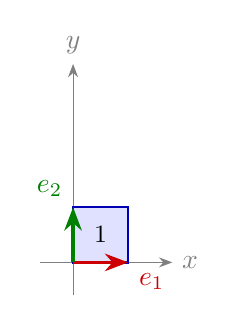
\begin{tikzpicture}[x=0.7cm, y=0.7cm, >=Stealth, baseline=(current bounding box.center)]
        \draw[->, gray] (-0.6,0) -- (1.8,0) node[right] {$x$};
        \draw[->, gray] (0,-0.6) -- (0,3.6) node[above] {$y$};
        \fill[blue!12] (0,0) -- (1,0) -- (1,1) -- (0,1) -- cycle;
        \draw[blue!70!black, thick] (0,0) -- (1,0) -- (1,1) -- (0,1) -- cycle;
        \draw[->, very thick, red!80!black] (0,0) -- (1,0) node[below right] {$e_1$};
        \draw[->, very thick, green!50!black] (0,0) -- (0,1) node[above left] {$e_2$};
        \node[font=\small] at (0.5,0.5) {$1$};
    \end{tikzpicture}
    \quad $\xrightarrow{\quad T_A \quad}$ \quad
    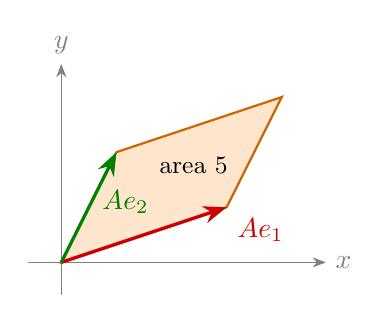
\begin{tikzpicture}[x=0.7cm, y=0.7cm, >=Stealth, baseline=(current bounding box.center)]
        \draw[->, gray] (-0.6,0) -- (4.8,0) node[right] {$x$};
        \draw[->, gray] (0,-0.6) -- (0,3.6) node[above] {$y$};
        \fill[orange!20] (0,0) -- (3,1) -- (4,3) -- (1,2) -- cycle;
        \draw[orange!80!black, thick] (0,0) -- (3,1) -- (4,3) -- (1,2) -- cycle;
        \draw[->, very thick, red!80!black] (0,0) -- (3,1) node[below right] {$Ae_1$};
        \draw[->, very thick, green!50!black] (0,0) -- (1,2) node[pos=0.55, right] {$Ae_2$};
        \node[font=\small] at (2.4,1.75) {area $5$};
    \end{tikzpicture}
    \caption[The determinant as an area]{The matrix $A$ with columns $(3, 1)$ and $(1, 2)$ maps the unit square (left, area $1$) to the parallelogram spanned by its columns $Ae_1$ and $Ae_2$ (right). The area of this parallelogram is $|\det(A)| = |3 \cdot 2 - 1 \cdot 1| = 5$.}
    \label{fig:det-area}
\end{figure}

\begin{figure}[ht]
    \centering
    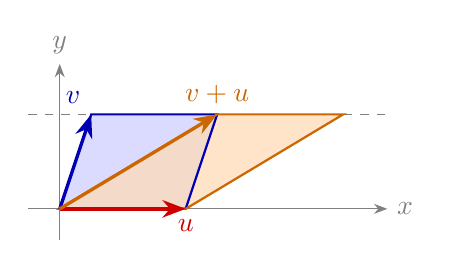
\begin{tikzpicture}[x=0.8cm, y=0.8cm, >=Stealth]
        \draw[->, gray] (-0.5,0) -- (5.2,0) node[right] {$x$};
        \draw[->, gray] (0,-0.5) -- (0,2.3) node[above] {$y$};
        \draw[gray, dashed] (-0.5,1.5) -- (5.2,1.5);
        \fill[blue!20, opacity=0.7] (0,0) -- (2,0) -- (2.5,1.5) -- (0.5,1.5) -- cycle;
        \fill[orange!30, opacity=0.7] (0,0) -- (2,0) -- (4.5,1.5) -- (2.5,1.5) -- cycle;
        \draw[blue!70!black, thick] (0,0) -- (2,0) -- (2.5,1.5) -- (0.5,1.5) -- cycle;
        \draw[orange!80!black, thick] (0,0) -- (2,0) -- (4.5,1.5) -- (2.5,1.5) -- cycle;
        \draw[->, very thick, red!80!black] (0,0) -- (2,0) node[below] {$u$};
        \draw[->, very thick, blue!70!black] (0,0) -- (0.5,1.5) node[above left] {$v$};
        \draw[->, very thick, orange!80!black] (0,0) -- (2.5,1.5) node[above] {$v + u$};
    \end{tikzpicture}
    \caption[Adding one column to another does not change the area]{The parallelograms spanned by $u = (2, 0)$ and $v = (\frac{1}{2}, \frac{3}{2})$ (blue) and by $u$ and $v + u$ (orange) have the same base $u$ and the same height (dashed line), hence the same area $3$. Correspondingly, adding the first column to the second column does not change the determinant: both matrices with these columns have determinant $2 \cdot \frac{3}{2} = 3$.}
    \label{fig:det-shear}
\end{figure}

\begin{example}
    \begin{itemize}
        \item $\det(\diag(2, 3)) = 6$: stretching by a factor $2$ in the $x$-direction and by a factor $3$ in the $y$-direction multiplies areas by $6$.
        \item $\det(R_\theta) = \cos^2\theta + \sin^2\theta = 1$: rotations preserve areas and orientation.
        \item $\det \begin{pmatrix} 1 & 0 \\ 0 & -1 \end{pmatrix} = -1$: the reflection in the $x$-axis preserves areas, but reverses orientation.
        \item $\det \begin{pmatrix} 1 & 2 \\ 2 & 4 \end{pmatrix} = 0$: this singular matrix maps the whole plane onto the line spanned by $(1, 2)$, which has area $0$ (see Figure~\ref{fig:kernel-image}).
    \end{itemize}
    Compare also with the gallery in Figure~\ref{fig:gallery}. The stretch (a) has determinant $\det \begin{pmatrix} 2 & 0 \\ 0 & 1 \end{pmatrix} = 2$ and doubles areas. The rotation (b) and the shear (d) have determinants $\det \begin{pmatrix} 0 & -1 \\ 1 & 0 \end{pmatrix} = 1$ and $\det \begin{pmatrix} 1 & 1 \\ 0 & 1 \end{pmatrix} = 1$: they preserve areas, even though the shear changes the shape of the square. The reflection (c) has determinant $-1$, which is why the image of the letter F is mirrored.
\end{example}

\subsubsection{Determinants, invertibility and products}

We now connect determinants with the inverse of a matrix, using the elementary matrices of Subsection~\ref{subsec:inverse}.

\begin{lemma}\label{lem:det-elementary}
    Let $E$ be an $n \times n$ elementary matrix. Then $\det(E) = -1$ if $E$ swaps two rows, $\det(E) = c$ if $E$ multiplies a row by $c \neq 0$, and $\det(E) = 1$ if $E$ adds a multiple of one row to another row. In all cases, $\det(E) \neq 0$, and
    \[\det(EA) = \det(E) \det(A) \qquad \text{for every } n \times n \text{ matrix } A.\]
\end{lemma}

\begin{proof}
    The matrix $E$ is obtained from $I_n$ by the row operation, and $\det(I_n) = 1$, so the values of $\det(E)$ follow from part 3 of Theorem~\ref{thm:det-props}. By Lemma~\ref{lem:elementary}, $EA$ is obtained from $A$ by the same row operation, so $\det(EA)$ is $\det(A)$ multiplied by $-1$, by $c$, or by $1$, respectively. In each case, this is $\det(E) \det(A)$.
\end{proof}

\begin{theorem}\label{thm:det-invertible}
    An $n \times n$ matrix $A$ is invertible if and only if $\det(A) \neq 0$.
\end{theorem}

\begin{proof}
    Let $E_1, \ldots, E_k$ be the elementary matrices of row operations that bring $A$ to $R = \RREF(A)$, so that $R = E_k \cdots E_1 A$. Applying Lemma~\ref{lem:det-elementary} $k$ times gives
    \[\det(R) = \det(E_k) \cdots \det(E_1) \det(A),\]
    where all the factors $\det(E_i)$ are nonzero. So $\det(A) \neq 0$ if and only if $\det(R) \neq 0$. If $A$ is invertible, then $R = I_n$ by Theorem~\ref{thm:invertible}, and $\det(R) = 1 \neq 0$. If $A$ is not invertible, then $R \neq I_n$, so $R$ has a row of zeros (as we saw after Theorem~\ref{thm:gauss-jordan}), and $\det(R) = 0$ by Corollary~\ref{cor:det-easy}.
\end{proof}

\begin{theorem}[Product rule]\label{thm:det-product}
    For all $n \times n$ matrices $A$ and $B$, we have $\det(AB) = \det(A) \det(B)$.
\end{theorem}

\begin{proof}
    Suppose first that $A$ is not invertible, so that $\det(A) = 0$ by Theorem~\ref{thm:det-invertible}. Then $AB$ is not invertible either: otherwise, $X = B(AB)^{-1}$ would satisfy $AX = I_n$, and by Corollary~\ref{cor:one-sided}, $X$ would be invertible with $X^{-1} = A$, so $A$ would be invertible. Hence $\det(AB) = 0 = \det(A) \det(B)$.

    Now suppose that $A$ is invertible. By the proof of Theorem~\ref{thm:invertible}, $A = (E_k \cdots E_1)^{-1} = E_1^{-1} \cdots E_k^{-1}$ for some elementary matrices $E_1, \ldots, E_k$, and each $F_i = E_i^{-1}$ is again an elementary matrix by Lemma~\ref{lem:elem-inv}. Applying Lemma~\ref{lem:det-elementary} $k$ times, we get
    \[\det(AB) = \det(F_1 F_2 \cdots F_k B) = \det(F_1) \det(F_2) \cdots \det(F_k) \det(B).\]
    Taking $B = I_n$ gives $\det(A) = \det(F_1) \cdots \det(F_k)$, and hence $\det(AB) = \det(A) \det(B)$.
\end{proof}

\begin{corollary}\label{cor:det-consequences}
    Let $A$ be an $n \times n$ matrix.
    \begin{enumerate}
        \item If $A$ is invertible, then $\det(A^{-1}) = 1/\det(A)$.
        \item If $P$ is an invertible $n \times n$ matrix, then $\det(P^{-1}AP) = \det(A)$.
        \item If $A$ is orthogonal, then $\det(A) = 1$ or $\det(A) = -1$.
    \end{enumerate}
\end{corollary}

\begin{proof}
    (1) $\det(A) \det(A^{-1}) = \det(AA^{-1}) = \det(I_n) = 1$.

    (2) $\det(P^{-1}AP) = \det(P^{-1}) \det(A) \det(P) = \det(A)$, by part 1.

    (3) $1 = \det(I_n) = \det(A^\top A) = \det(A^\top) \det(A) = \det(A)^2$.
\end{proof}

\begin{remark}
    Unlike the trace, the determinant is not linear. For example, $\det(I_2 + I_2) = \det(2I_2) = 4$, while $\det(I_2) + \det(I_2) = 2$.
\end{remark}

\begin{example}[Inverse of a $2 \times 2$ matrix]
    Let $A = \begin{pmatrix} a & b \\ c & d \end{pmatrix}$ with $\det(A) = ad - bc \neq 0$. Then
    \[A^{-1} = \frac{1}{ad - bc} \begin{pmatrix}
        d & -b \\
        -c & a
    \end{pmatrix}.\]
    Indeed,
    \[\begin{pmatrix}
        a & b \\
        c & d
    \end{pmatrix} \begin{pmatrix}
        d & -b \\
        -c & a
    \end{pmatrix} = \begin{pmatrix}
        ad - bc & 0 \\
        0 & ad - bc
    \end{pmatrix} = (ad - bc) I_2,\]
    and by Corollary~\ref{cor:one-sided}, checking one product is enough. For example, for the matrix of Example~\ref{ex:inverse2x2}, with determinant $-14$,
    \[\begin{pmatrix}
        2 & 3 \\
        4 & -1
    \end{pmatrix}^{-1} = \frac{1}{-14} \begin{pmatrix}
        -1 & -3 \\
        -4 & 2
    \end{pmatrix} = \frac{1}{14} \begin{pmatrix}
        1 & 3 \\
        4 & -2
    \end{pmatrix},\]
    as we found before. For larger matrices, there is a similar formula, $A^{-1} = \frac{1}{\det(A)} C^\top$, where $C$ is the matrix of cofactors $C_{ij}$; we do not prove it here. For computations, the Gauss--Jordan method is much more efficient.
\end{example}

Theorem~\ref{thm:det-invertible} says that $\mathrm{GL}(n, \mathbb{R}) = \{A \in \mathbb{R}^{n \times n} : \det(A) \neq 0\}$. Determinants also give us another matrix group.

\begin{definition}[Special linear group]
    The special linear group is the set
    \[\mathrm{SL}(n, \mathbb{R}) = \{A \in \mathbb{R}^{n \times n} : \det(A) = 1\}.\]
\end{definition}

\begin{proposition}
    The set $\mathrm{SL}(n, \mathbb{R})$ is contained in $\mathrm{GL}(n, \mathbb{R})$ and is not a subspace of $\mathbb{R}^{n \times n}$. However, it contains $I_n$ and is closed under multiplication and under taking inverses, so it is a matrix group.
\end{proposition}

\begin{proof}
    Every matrix with determinant $1$ is invertible by Theorem~\ref{thm:det-invertible}. The zero matrix has determinant $0$, so it is not in $\mathrm{SL}(n, \mathbb{R})$, and $\mathrm{SL}(n, \mathbb{R})$ is not a subspace. We have $\det(I_n) = 1$. If $\det(A) = \det(B) = 1$, then $\det(AB) = 1 \cdot 1 = 1$ by Theorem~\ref{thm:det-product}, and $\det(A^{-1}) = 1/1 = 1$ by Corollary~\ref{cor:det-consequences}.
\end{proof}

\begin{example}
    All rotation matrices $R_\theta$ belong to $\mathrm{SL}(2, \mathbb{R})$, and so does $\diag(2, \frac{1}{2})$, which stretches the plane by a factor $2$ in one direction and shrinks it by a factor $2$ in the other. By the geometric meaning of the determinant, the matrices in $\mathrm{SL}(2, \mathbb{R})$ are exactly the $2 \times 2$ matrices whose linear transformations preserve areas and orientation.
\end{example}

\section{Null Space, Column Space and Rank}

Row reduction is our main tool for computing the kernel and the image of a linear transformation $T: \mathbb{R}^n \to \mathbb{R}^m$. To use it, we first introduce the corresponding notions for matrices.

\begin{definition}
    Let $A$ be an $m \times n$ matrix.

    The null space of $A$ is the set of all vectors $x \in \mathbb{R}^n$ such that $Ax = 0$. It is denoted as $\Null(A)$. If $T(x) = Ax$, then $\Null(A) = \ker(T)$.

    The column space of $A$ is the set of all linear combinations of the columns of $A$. It is denoted as $\col(A)$. By Remark~\ref{rem:columns}, the vectors $Ax$ are exactly the linear combinations of the columns of $A$, so if $T(x) = Ax$, then $\col(A) = \im(T)$.

    The row space of $A$ is the set of all linear combinations of the rows of $A$. It is denoted as $\row(A)$. Writing the rows as columns, $\row(A) = \col(A^\top)$, which is the image of the linear transformation represented by the transpose $A^\top$.
\end{definition}

By Theorem~\ref{thm:kerim}, $\Null(A)$ is a subspace of $\mathbb{R}^n$ and $\col(A)$ is a subspace of $\mathbb{R}^m$. The following theorem explains how row reduction affects these spaces.

\begin{theorem}\label{thm:rowops}
    Let $A$ be an $m \times n$ matrix, and let $R$ be obtained from $A$ by a sequence of elementary row operations. Then:
    \begin{enumerate}
        \item $\Null(A) = \Null(R)$, i.e., the equations $Ax = 0$ and $Rx = 0$ have exactly the same solutions;
        \item $\row(A) = \row(R)$;
        \item if $R = \RREF(A)$, then the columns of $A$ in the positions of the pivot columns of $R$ (the pivot columns of $A$) form a basis of $\col(A)$.
    \end{enumerate}
\end{theorem}

\begin{proof}
    It is enough to consider a single elementary row operation, since we can then repeat the argument for each operation in the sequence.

    (1) Each equation of the new system is a linear combination of the equations of the old system, so every solution of the old system is also a solution of the new one. Since the operation can be undone by another elementary row operation, the converse holds as well.

    (2) Similarly, every row of the new matrix is a linear combination of the rows of the old matrix, so the new row space is contained in the old one. Undoing the operation shows the reverse inclusion.

    (3) Let $a_1, \ldots, a_n$ be the columns of $A$ and $r_1, \ldots, r_n$ the columns of $R$. For any scalars $c_1, \ldots, c_n$, part (1) applied to $c = (c_1, \ldots, c_n)^\top$ gives
    \[c_1 a_1 + \cdots + c_n a_n = 0 \iff Ac = 0 \iff Rc = 0 \iff c_1 r_1 + \cdots + c_n r_n = 0.\]
    So the columns of $A$ satisfy exactly the same linear relations as the columns of $R$. If $R$ has $r$ pivots, then its pivot columns are the standard basis vectors $e_1, \ldots, e_r$ of $\mathbb{R}^m$, which are linearly independent. Every other column of $R$ has zeros in its last $m - r$ entries, so it is a linear combination of $e_1, \ldots, e_r$. Transferring these relations back to $A$, the pivot columns of $A$ are linearly independent, and every other column of $A$ is a linear combination of them. Hence the pivot columns of $A$ span $\col(A)$, and they form a basis of $\col(A)$.
\end{proof}

\begin{remark}
    Elementary row operations can change the column space! For example,
    \[\begin{pmatrix}
        1 & 1 \\
        1 & 1
    \end{pmatrix} \quad \xrightarrow{\text{subtract row 1 from row 2}} \quad \begin{pmatrix}
        1 & 1 \\
        0 & 0
    \end{pmatrix},\]
    but the column space of the first matrix is $\Span\{(1, 1)^\top\}$, while the column space of the second matrix is $\Span\{(1, 0)^\top\}$. This is why, in part 3 of Theorem~\ref{thm:rowops}, we take the pivot columns of the original matrix $A$, not of $R$.
\end{remark}

\begin{example}\label{ex:worked}
    Consider again the linear transformation $T: \mathbb{R}^3 \to \mathbb{R}^2$ defined by $T(x, y, z) = (x + 2y - z, 3x - y + 4z)$. The matrix representation of $T$ is
    \[A = \begin{pmatrix}
        1 & 2 & -1 \\
        3 & -1 & 4
    \end{pmatrix}.\]

    We will transform this matrix into reduced row echelon form to find the null space, column space and row space of $A$, and hence the kernel and image of $T$.

    First, we can eliminate the leading entry in the second row by subtracting $3$ times the first row from the second row:
    \[\begin{pmatrix}
        1 & 2 & -1 \\
        0 & -7 & 7
    \end{pmatrix}.\]

    Next, we can multiply the second row by $-1/7$ to make the leading entry of the second row equal to $1$:
    \[\begin{pmatrix}
        1 & 2 & -1 \\
        0 & 1 & -1
    \end{pmatrix}.\]

    Now we can eliminate the entry above the leading $1$ in the second row by subtracting $2$ times the second row from the first row:
    \[\RREF(A) = \begin{pmatrix}
        1 & 0 & 1 \\
        0 & 1 & -1
    \end{pmatrix}.\]

    \textbf{Null space.} By Theorem~\ref{thm:rowops}, the equation $Ax = 0$, where $x = (x_1, x_2, x_3)^\top$, has the same solutions as $\RREF(A)\,x = 0$. From the RREF, we have:
    \begin{align*}
        x_1 + x_3 &= 0 \implies x_1 = -x_3, \\
        x_2 - x_3 &= 0 \implies x_2 = x_3.
    \end{align*}

    Letting $x_3 = t$ for some scalar $t$, we have:
    \[x = (-t, t, t)^\top = t(-1, 1, 1)^\top.\]
    Therefore, $\ker(T) = \Null(A) = \Span\{(-1, 1, 1)^\top\}$. This agrees with Example~\ref{ex:ker2}, where we found $\ker(T) = \{(x, -x, -x) : x \in \mathbb{R}\}$ (take $x = -t$).

    \textbf{Column space.} The pivots of $\RREF(A)$ are in columns $1$ and $2$. By Theorem~\ref{thm:rowops}, the first two columns of the original matrix $A$,
    \[\begin{pmatrix}
        1 \\
        3
    \end{pmatrix}, \quad
    \begin{pmatrix}
        2 \\
        -1
    \end{pmatrix},\]
    form a basis of $\col(A)$. These two vectors span all of $\mathbb{R}^2$, since every $(u, v)^\top \in \mathbb{R}^2$ can be written as
    \[\begin{pmatrix}
        u \\
        v
    \end{pmatrix} = \frac{u + 2v}{7} \begin{pmatrix}
        1 \\
        3
    \end{pmatrix} + \frac{3u - v}{7} \begin{pmatrix}
        2 \\
        -1
    \end{pmatrix}.\]
    Hence $\im(T) = \col(A) = \mathbb{R}^2$, which agrees with Example~\ref{ex:im2}.

    \textbf{Row space.} By Theorem~\ref{thm:rowops}, $\row(A) = \row(\RREF(A))$, so the row space of $A$ is spanned by the nonzero rows of the RREF:
    \[\begin{pmatrix}
        1 & 0 & 1
    \end{pmatrix}, \quad
    \begin{pmatrix}
        0 & 1 & -1
    \end{pmatrix}.\]
    These two rows are linearly independent (look at their first two entries), so they form a basis of $\row(A)$.
\end{example}

\begin{definition}[Rank]
    The rank of a matrix $A$ is the dimension of its column space, $\rank(A) = \dim \col(A)$. If $T(x) = Ax$, this is the dimension of the image of $T$.
\end{definition}

\begin{theorem}\label{thm:rank}
    Let $A$ be a matrix, and let $r$ be the number of pivots of $\RREF(A)$, which is the same as the number of nonzero rows of $\RREF(A)$. Then
    \[\rank(A) = r = \dim \row(A).\]
\end{theorem}

\begin{proof}
    By part 3 of Theorem~\ref{thm:rowops}, the $r$ pivot columns of $A$ form a basis of $\col(A)$, so $\rank(A) = r$.

    By part 2 of Theorem~\ref{thm:rowops}, the $r$ nonzero rows of $\RREF(A)$ span $\row(A)$. They are also linearly independent: each of them has a $1$ in its pivot column, where all the other rows have a $0$. So they form a basis of $\row(A)$, and $\dim \row(A) = r$.
\end{proof}

\begin{remark}
    In practice, $\rank(A)$ is the number of nonzero rows in any row echelon form of $A$: clearing the entries above the leading $1$s, as in Examples~\ref{ex:G} and~\ref{ex:H}, turns a row echelon form into the RREF without changing the number of nonzero rows. Also, Theorem~\ref{thm:rank} says that $\dim \col(A) = \dim \row(A)$: a matrix has as many linearly independent columns as linearly independent rows. This is far from obvious!
\end{remark}

\begin{example}
    Consider the matrix
    \[M = \begin{pmatrix}
        1 & 2 & 3 \\
        0 & 1 & 4 \\
        0 & 0 & 0
    \end{pmatrix}.\]
    This matrix is already in row echelon form. The number of nonzero rows is $2$, so the rank of the matrix $M$ is $\rank(M) = 2$. Similarly, the matrix $A$ in Example~\ref{ex:worked} has rank $2$.
\end{example}

\begin{theorem}[Rank--nullity theorem]
    For any $m \times n$ matrix $A$,
    \[\rank(A) + \dim \Null(A) = n.\]
    Equivalently, if $T: \mathbb{R}^n \to \mathbb{R}^m$ is a linear transformation, then $\dim \im(T) + \dim \ker(T) = n$.
\end{theorem}

\begin{proof}[Idea of proof]
    Let $r$ be the number of pivots of $\RREF(A)$, so that $\rank(A) = r$ by Theorem~\ref{thm:rank}. When we solve $\RREF(A)\,x = 0$, the $r$ variables corresponding to the pivot columns are expressed in terms of the remaining $n - r$ free variables. Setting one free variable equal to $1$ and all others equal to $0$ gives $n - r$ solutions. Every solution is a linear combination of these, and they are linearly independent, since each of them has a $1$ in a position where all the others have a $0$. So they form a basis of $\Null(A)$, and $\dim \Null(A) = n - r$.
\end{proof}

\begin{example}
    For $T(x, y, z) = (x + 2y - z, 3x - y + 4z)$, we found in Example~\ref{ex:worked} that $\dim \ker(T) = 1$ and $\dim \im(T) = 2$, and indeed $2 + 1 = 3 = n$. For $T(x, y) = (2x + 3y, 4x - y)$, we found in Examples~\ref{ex:ker1} and~\ref{ex:im1} that $\ker(T) = \{(0, 0)\}$, of dimension $0$, and $\im(T) = \mathbb{R}^2$, of dimension $2$; indeed $2 + 0 = 2 = n$.
\end{example}

Combining the rank--nullity theorem with Theorem~\ref{thm:invertible}, we obtain several ways to recognize an invertible matrix.

\begin{corollary}\label{cor:invertible-rank}
    For an $n \times n$ matrix $A$, the following statements are equivalent:
    \begin{enumerate}
        \item $A$ is invertible;
        \item $\Null(A) = \{0\}$;
        \item $\rank(A) = n$;
        \item for every $b \in \mathbb{R}^n$, the equation $Ax = b$ has exactly one solution;
        \item $\det(A) \neq 0$.
    \end{enumerate}
\end{corollary}

\begin{proof}
    Statements 1 and 2 are equivalent by Theorem~\ref{thm:invertible}. By the rank--nullity theorem, $\rank(A) = n - \dim \Null(A)$, so $\rank(A) = n$ if and only if $\dim \Null(A) = 0$, i.e., $\Null(A) = \{0\}$; hence statements 2 and 3 are equivalent. Statement 1 implies statement 4 by Remark~\ref{rem:inverse-solve}, and statement 4 implies statement 2 by taking $b = 0$. Finally, statements 1 and 5 are equivalent by Theorem~\ref{thm:det-invertible}.
\end{proof}

\begin{exercise}
    Let $T: \mathbb{R}^2 \to \mathbb{R}^2$ be defined by $T(x, y) = (x - y, 2x + 3y)$. Find the kernel and image of $T$, and check that your answer agrees with the rank--nullity theorem.
\end{exercise}

\section{Key Takeaways}
\begin{itemize}[leftmargin=*]
	\item A field is a set of ``numbers'' in which we can add, subtract, multiply, and divide by nonzero elements. $\mathbb{Q}$, $\mathbb{R}$ and $\mathbb{C}$ are fields; $\mathbb{Z}$ is not.
	\item A vector space over a field $\mathbb{F}$ is a set of vectors that can be added and multiplied by scalars from $\mathbb{F}$, subject to the vector space axioms. Examples: $\mathbb{F}$ itself, products $V \times W$, $\mathbb{R}^n$, and the polynomials $\mathbb{R}[x]$.
	\item A basis is a linearly independent set that spans the space; every vector is a unique linear combination of the basis vectors. All bases of a finite-dimensional space have the same number of vectors, the dimension: $\dim \mathbb{R}^n = n$, while $\mathbb{R}[x]$ is infinite-dimensional.
	\item A linear transformation $T: V \to W$ preserves addition and scalar multiplication, and $T(0_V) = 0_W$. Its kernel is a subspace of $V$, and its image is a subspace of $W$.
	\item An isomorphism is a bijective linear transformation, i.e., one with $\ker(T) = \{0\}$ and $\im(T) = W$. Via coordinates, every $n$-dimensional real vector space is isomorphic to $\mathbb{R}^n$, and $V \cong W$ if and only if $\dim V = \dim W$, if and only if some linear transformation $V \to W$ is represented by an invertible matrix.
	\item Every linear transformation $T: \mathbb{R}^n \to \mathbb{R}^m$ is multiplication by an $m \times n$ matrix $A$, whose $i$-th column is $T(e_i)$.
	\item Matrices of the same size are added entry by entry. The product of an $m \times n$ and an $n \times p$ matrix is the $m \times p$ matrix with $(AB)_{ij} = \sum_k A_{ik} B_{kj}$; it represents the composition $T_A \circ T_B$. Matrix multiplication is associative but not commutative, and $(AB)^\top = B^\top A^\top$.
	\item A square matrix $A$ is invertible if $AB = BA = I_n$ for some matrix $B = A^{-1}$; then $Ax = b$ has the unique solution $x = A^{-1}b$, and $(AB)^{-1} = B^{-1}A^{-1}$. The inverse is computed without determinants by row reducing $(A \mid I_n)$ to $(I_n \mid A^{-1})$.
	\item Diagonal, upper and lower triangular, symmetric ($A^\top = A$) and skew-symmetric ($A^\top = -A$) matrices form subspaces of $\mathbb{R}^{n \times n}$. The invertible matrices $\mathrm{GL}(n, \mathbb{R})$ and the orthogonal matrices $\mathrm{O}(n)$ (with $Q^\top Q = I_n$, so $Q^{-1} = Q^\top$) do not form subspaces, but they contain $I_n$ and are closed under multiplication and inverses: they are matrix groups.
	\item The trace $\tr(A) = \sum_i A_{ii}$ is linear and satisfies $\tr(AB) = \tr(BA)$. The determinant is defined by cofactor expansion and is best computed by row reduction to triangular form; it satisfies $\det(AB) = \det(A)\det(B)$ and $\det(A^\top) = \det(A)$, and $|\det(A)|$ is the factor by which $T_A$ scales areas and volumes.
	\item Elementary row operations bring a matrix into (reduced) row echelon form. They do not change the null space or the row space, but they can change the column space; the pivot columns of the original matrix form a basis of its column space.
	\item $\rank(A) = \dim \col(A) = \dim \row(A)$ is the number of pivots, and $\rank(A) + \dim \Null(A) = n$ for every $m \times n$ matrix $A$.
	\item For an $n \times n$ matrix $A$: $A$ is invertible $\iff$ $\Null(A) = \{0\}$ $\iff$ $\rank(A) = n$ $\iff$ $\RREF(A) = I_n$ $\iff$ $\det(A) \neq 0$.
\end{itemize}

\section{Exercises}\label{sec:exercises}
\begin{enumerate}[leftmargin=*]
	\item\label{ex:axioms} Using only the vector space axioms, prove that in every vector space $V$ over a field $\mathbb{F}$:
	\begin{enumerate}
		\item $0 \cdot v = 0_V$ for every $v \in V$. (Hint: $0 \cdot v = (0 + 0) \cdot v$.)
		\item $(-1) \cdot v = -v$ for every $v \in V$. (Hint: compute $v + (-1) \cdot v$.)
	\end{enumerate}
	\item Which of the following subsets of $\mathbb{R}^2$ are subspaces? Justify your answers.
	\begin{enumerate}
		\item $\{(x, y) \in \mathbb{R}^2 : y = 2x\}$;
		\item $\{(x, y) \in \mathbb{R}^2 : y = 2x + 1\}$;
		\item $\{(x, y) \in \mathbb{R}^2 : xy = 0\}$.
	\end{enumerate}
	\item Show that $\{(1, 2), (3, 4)\}$ is a basis of $\mathbb{R}^2$, and write $(5, 6)$ as a linear combination of these two vectors.
	\item Let $\mathbb{R}[x]_{\leq 2}$ be the set of polynomials with real coefficients of degree at most $2$. Show that it is a subspace of $\mathbb{R}[x]$, and find its dimension.
	\item Let $T: \mathbb{R}^3 \to \mathbb{R}^3$ be defined by $T(x, y, z) = (x + y, y + z, x + 2y + z)$. Find the matrix $A$ of $T$ and $\RREF(A)$. Then find a basis of $\Null(A)$, a basis of $\col(A)$, and $\rank(A)$, and check that your answers agree with the rank--nullity theorem.
	\item Write down explicit isomorphisms $\mathbb{R}^{2 \times 2} \to \mathbb{R}^4$ and $\mathrm{Sym}_2 \to \mathbb{R}^3$, and prove that they are isomorphisms. Are $\mathbb{R}^{2 \times 2}$ and $\mathrm{Sym}_2$ isomorphic?
	\item Let $A = \begin{pmatrix} 1 & 2 \\ 3 & 4 \end{pmatrix}$ and $B = \begin{pmatrix} 0 & 1 \\ 1 & 0 \end{pmatrix}$. Compute $AB$ and $BA$. Describe in words what multiplying a $2 \times 2$ matrix by $B$ from the left does, and what multiplying it by $B$ from the right does.
	\item Use the Gauss--Jordan method to find the inverse of
	\[A = \begin{pmatrix}
		1 & 2 & 3 \\
		0 & 1 & 4 \\
		5 & 6 & 0
	\end{pmatrix},\]
	and check your answer.
	\item Show that the matrix $F$ from Example~\ref{ex:F} is not invertible, and find a nonzero vector $x$ with $Fx = 0$.
	\item Let $A$ be an $n \times n$ matrix with $A^2 = A$ (where $A^2 = AA$) and $A \neq I_n$. Show that $A$ is not invertible.
	\item Show that an upper triangular matrix is invertible if and only if all of its diagonal entries are nonzero, in two ways: using Theorem~\ref{thm:invertible}, and using determinants.
	\item Compute the determinant of
	\[A = \begin{pmatrix}
		2 & 0 & 1 \\
		1 & 3 & 2 \\
		1 & 1 & 1
	\end{pmatrix}\]
	in two ways: by cofactor expansion, and by row reduction. Is $A$ invertible?
	\item Let $A$ be a skew-symmetric $n \times n$ matrix, where $n$ is odd. Show that $\det(A) = 0$. (Hint: compute $\det(A^\top)$ in two ways.)
	\item Show that $\tr(ABC) = \tr(CAB)$ for all $n \times n$ matrices $A$, $B$, $C$, but find $2 \times 2$ matrices with $\tr(ABC) \neq \tr(ACB)$.
\end{enumerate}

\section{Programming Exercises}\label{sec:programming}

% Inline code cannot be hyphenated, so allow a little extra stretch in this section.
\setlength{\emergencystretch}{3em}

In these exercises, you implement the main algorithms of this lecture in Python. You need Python~3 with NumPy, and Matplotlib for Exercise~P6. Implement the algorithms yourself, using only loops, indexing and arithmetic on NumPy arrays; use NumPy's built-in linear algebra routines (\py{np.linalg}) only to check your results. Start each file with
\begin{lstlisting}
import numpy as np
rng = np.random.default_rng(0)  # random number generator for test matrices
\end{lstlisting}

\paragraph{A word on floating-point numbers.} Computers store real numbers with only about $16$ significant digits, so almost every computation has tiny rounding errors; for example, \py{0.1 + 0.2 == 0.3} is \py{False} in Python. Therefore, never test whether a computed number is exactly zero: test \py{abs(x) < tol} for a small tolerance such as \py{tol = 1e-10} instead, and compare arrays with \py{np.allclose(X, Y)}. Also remember that Python counts from $0$: the entry $A_{ij}$ of these notes is \py{A[i-1, j-1]} in NumPy.

\begin{enumerate}[label=\textbf{P\arabic*.}, leftmargin=*]
    \item \textbf{Matrices of linear transformations.} Write a function that takes a linear transformation $T: \mathbb{R}^n \to \mathbb{R}^m$, given as a Python function that maps NumPy vectors of length $n$ to vectors of length $m$, and returns its $m \times n$ matrix, whose $i$-th column is $T(e_i)$ (Theorem~\ref{thm:matrix}).
\begin{lstlisting}
def matrix_of(T, n):
    """Return the matrix of the linear transformation T: R^n -> R^m."""
    ...

T = lambda v: np.array([2*v[0] + 3*v[1], 4*v[0] - v[1]])
print(matrix_of(T, 2))  # should print [[ 2.  3.] [ 4. -1.]]
\end{lstlisting}
    \begin{itemize}
        \item Also test your function on $T(x, y, z) = (x + 2y - z, 3x - y + 4z)$, and compare with the matrix computed in the examples after Theorem~\ref{thm:matrix}.
        \item Write a function \py{looks_linear(T, n, trials=100)} that checks additivity and homogeneity for random vectors \py{u = rng.normal(size=n)}, \py{v = rng.normal(size=n)} and random scalars \py{a = rng.normal()}. Test it on the $T$ above and on the maps $(x, y) \mapsto (x + 1, y)$ and $(x, y) \mapsto (xy, y)$.
        \item Why can such a random test prove that a map is \emph{not} linear, but never prove that a map \emph{is} linear?
    \end{itemize}

    \item \textbf{Matrix multiplication from scratch.} Implement \py{matmul(A, B)} with three nested loops, directly from the definition $(AB)_{ij} = \sum_k A_{ik} B_{kj}$. Raise a \py{ValueError} if the number of columns of \py{A} is not equal to the number of rows of \py{B}.
    \begin{itemize}
        \item Compare \py{matmul(A, B)} with NumPy's \py{A @ B} for random matrices of several shapes.
        \item Use your function to check numerically that $(AB)C = A(BC)$ and $(AB)^\top = B^\top A^\top$ (Proposition~\ref{prop:mult-props}), and find random $2 \times 2$ matrices with $AB \neq BA$.
        \item Measure the running times (with \py{time.perf_counter()}) of \py{matmul} and of \py{@} for random $n \times n$ matrices with $n = 50, 100, 200$. By roughly what factor does the running time of \py{matmul} grow when $n$ doubles? Explain this by counting the multiplications that are performed. (NumPy is much faster because it runs highly optimized compiled code.)
    \end{itemize}

    \item \textbf{Row reduction.} Implement a function that computes the reduced row echelon form of a matrix and its pivot columns.
\begin{lstlisting}
def rref(A, tol=1e-10):
    """Return (R, pivots): the RREF of A and the list of pivot columns."""
    R = np.array(A, dtype=float)  # work on a copy of A
    ...
\end{lstlisting}
    Go through the columns from left to right, keeping track of the row $r$ in which the next pivot will be placed. For each column $c$, find the entry with the largest absolute value among the rows $r, r+1, \ldots$ of that column. If it is smaller than \py{tol}, the column has no pivot. Otherwise, swap its row with row $r$, divide row $r$ by the pivot, and subtract multiples of row $r$ from all the other rows so that all other entries of column $c$ become zero. (Choosing the largest available entry as the pivot is called partial pivoting; it reduces rounding errors.)
    \begin{itemize}
        \item Test your function: the matrix $\begin{pmatrix} 1 & 2 & -1 \\ 3 & -1 & 4 \end{pmatrix}$ should give $\begin{pmatrix} 1 & 0 & 1 \\ 0 & 1 & -1 \end{pmatrix}$ with pivots \py{[0, 1]}, and the matrix $F$ of Example~\ref{ex:F} should give $\begin{pmatrix} 1 & 0 & -1 \\ 0 & 1 & 2 \\ 0 & 0 & 0 \end{pmatrix}$.
        \item Using \py{rref}, write functions \py{rank(A)}, \py{null_space_basis(A)}, which returns one basis vector for each free variable as in the proof of the rank--nullity theorem, and \py{col_space_basis(A)}, which returns the pivot columns of the \emph{original} matrix (Theorem~\ref{thm:rowops}).
        \item For $20$ random $5 \times 7$ matrices $A$, check that \py{A @ v} is close to zero for every vector \py{v} in \py{null_space_basis(A)}, that \py{rank(A) + len(null_space_basis(A)) == 7} (rank--nullity), and that \py{rank(A)} agrees with \py{np.linalg.matrix_rank(A)}.
        \item Random matrices almost always have the largest possible rank. Construct a $6 \times 8$ matrix of rank $4$ as the product of a random $6 \times 4$ matrix and a random $4 \times 8$ matrix, and check that your functions find rank $4$ and a $4$-dimensional null space.
    \end{itemize}

    \item \textbf{The inverse with the Gauss--Jordan method.} Implement \py{inverse(A)}: row reduce the $n \times 2n$ matrix $(A \mid I_n)$ with your \py{rref} (use \py{np.hstack} and \py{np.eye}) and return the right block. If the left block is not $I_n$, raise \py{np.linalg.LinAlgError("matrix is singular")} (Theorem~\ref{thm:gauss-jordan}).
    \begin{itemize}
        \item Check your function on the examples of Subsection~\ref{subsec:inverse}: the inverse of $\begin{pmatrix} 2 & 3 \\ 4 & -1 \end{pmatrix}$ is $\frac{1}{14} \begin{pmatrix} 1 & 3 \\ 4 & -2 \end{pmatrix}$, the inverse of $\begin{pmatrix} 1 & 1 & 0 \\ 0 & 1 & 1 \\ 1 & 1 & 1 \end{pmatrix}$ is $\begin{pmatrix} 0 & -1 & 1 \\ 1 & 1 & -1 \\ -1 & 0 & 1 \end{pmatrix}$, and $\begin{pmatrix} 1 & 2 \\ 2 & 4 \end{pmatrix}$ is singular.
        \item For a random $10 \times 10$ matrix $A$, check that \py{A @ inverse(A)} and \py{inverse(A) @ A} are both close to $I_{10}$, and that \py{inverse(A)} is close to \py{np.linalg.inv(A)}.
    \end{itemize}

    \item \textbf{Determinants in two ways.} Implement \py{det_cofactor(A)}, which computes the determinant recursively by cofactor expansion along the first row (Subsection~\ref{subsec:trace-det}), and \py{det_rowreduce(A)}, which brings $A$ into upper triangular form by row operations, keeps track of the sign changes caused by row swaps, and multiplies the diagonal entries (Theorem~\ref{thm:det-props} and Corollary~\ref{cor:det-easy}). Hint: \py{np.delete(A[1:], j, axis=1)} is the matrix obtained from \py{A} by deleting its first row and the column with index \py{j}.
    \begin{itemize}
        \item Both functions should return $-3$ for $\begin{pmatrix} 1 & 2 & 3 \\ 4 & 5 & 6 \\ 7 & 8 & 10 \end{pmatrix}$, and $0$ (up to rounding) for the matrix $F$ of Example~\ref{ex:F}. Compare both functions with \py{np.linalg.det} on random matrices.
        \item Check the product rule $\det(AB) = \det(A) \det(B)$ and the rule $\det(A^\top) = \det(A)$ on random $5 \times 5$ matrices.
        \item Measure the running time of \py{det_cofactor} for random $n \times n$ matrices with $n = 2, 3, \ldots, 8$. By roughly what factor does it grow from $n - 1$ to $n$, and why? Estimate how long \py{det_cofactor} would need for $n = 20$, and compare with the running time of \py{det_rowreduce} for $n = 200$.
    \end{itemize}

    \item \textbf{Visualizing linear transformations.} Using Matplotlib, write a function that draws the unit square, a few grid lines inside it and the letter F, before and after applying a $2 \times 2$ matrix $A$, as in Figure~\ref{fig:gallery}.
\begin{lstlisting}
def plot_transformation(A):
    """Draw the unit square, a grid and the letter F, before and after A."""
    ...
\end{lstlisting}
    Store a shape as an array \py{P} with one point per row; then its image under $A$ is \py{P @ A.T}. The letter F in the figures has the corners
    \begin{gather*}
        (0.2, 0.1),\ (0.4, 0.1),\ (0.4, 0.45),\ (0.65, 0.45),\ (0.65, 0.6), \\
        (0.4, 0.6),\ (0.4, 0.75),\ (0.8, 0.75),\ (0.8, 0.9),\ (0.2, 0.9).
    \end{gather*}
    \begin{itemize}
        \item Reproduce the four panels of Figure~\ref{fig:gallery}, and also plot the singular matrix $\begin{pmatrix} 1 & 2 \\ 2 & 4 \end{pmatrix}$.
        \item The signed area of a polygon with corners $(x_1, y_1), \ldots, (x_k, y_k)$ is given by the shoelace formula
        \[\frac{1}{2} \sum_{i=1}^k (x_i y_{i+1} - x_{i+1} y_i), \qquad \text{where } (x_{k+1}, y_{k+1}) = (x_1, y_1).\]
        It is positive if the corners are listed counterclockwise, and negative if they are listed clockwise. Implement it, apply it to the image of the unit square with corners listed in the order $(0, 0), (1, 0), (1, 1), (0, 1)$, and check that the result equals $\det(A)$, including the sign, for all the matrices above and for the matrix $\begin{pmatrix} 3 & 1 \\ 1 & 2 \end{pmatrix}$ of Figure~\ref{fig:det-area}.
    \end{itemize}

    \item \textbf{Special matrices.}
    \begin{itemize}
        \item Write functions \py{is_symmetric(A, tol=1e-10)} and \py{is_orthogonal(Q, tol=1e-10)}.
        \item For a random $3 \times 5$ matrix $A$ and a random $5 \times 3$ matrix $B$, check that \py{A.T @ A} is symmetric, that $\tr(AB) = \tr(BA)$ (even though $AB$ and $BA$ have different sizes!), and that $\tr(A^\top A)$ equals \py{np.linalg.norm(A, "fro")**2}.
        \item Write a function that splits a square matrix into its symmetric and skew-symmetric parts (Exercise~\ref{exer:special}), and test it.
        \item The command \py{Q, R = np.linalg.qr(rng.normal(size=(4, 4)))} produces a random orthogonal matrix \py{Q}. Check that \py{Q} is orthogonal, that $\det(Q) = \pm 1$ (Corollary~\ref{cor:det-consequences}), and that $Q$ preserves lengths: \py{np.linalg.norm(Q @ x)} equals \py{np.linalg.norm(x)} for random vectors $x$, where the length of $x$ is $\sqrt{x_1^2 + \cdots + x_n^2}$.
    \end{itemize}

    \item \textbf{Why you should not compute the inverse.} The Hilbert matrix $H_n$ is the $n \times n$ matrix with entries $(H_n)_{ij} = \frac{1}{i + j - 1}$. It is invertible, but very close to being singular, which makes computations with it very sensitive to rounding errors. For $n = 4, 6, 8, 10, 12$, let \py{x_true = np.ones(n)} and \py{b = H @ x_true}, and solve $H_n x = b$ in three ways:
\begin{lstlisting}
x1 = np.linalg.solve(H, b)
x2 = np.linalg.inv(H) @ b
x3 = inverse(H) @ b  # your function from P4
\end{lstlisting}
    For each method, print the error $\max_i |x_i - 1|$ and the residual $\max_i |(H_n x - b)_i|$. What do you observe? Which method keeps the residual smallest? What happens with your own \py{inverse} for larger $n$, and why? (Hint: think about the tolerance in \py{rref}.) Relate your observations to Remark~\ref{rem:solve-practice}.

    \item \textbf{Mini-project: fitting a line to data.} Given data points $(x_1, y_1), \ldots, (x_N, y_N)$, we look for the line $y = w_0 + w_1 x$ that fits the data best, in the sense that the sum of squared errors $\sum_i (y_i - w_0 - w_1 x_i)^2$ is as small as possible. This is the simplest example of linear regression. Let $X$ be the $N \times 2$ matrix with rows $(1, x_i)$, and let $y = (y_1, \ldots, y_N)^\top$. One can show (we do not prove this here) that the best $w = (w_0, w_1)^\top$ is the solution of the normal equations
    \[(X^\top X)\, w = X^\top y.\]
    \begin{itemize}
        \item Generate data on a line with some noise:
\begin{lstlisting}
x = np.linspace(0, 1, 50)
y = 2 + 3 * x + rng.normal(0, 0.1, size=50)  # a line plus noise
X = np.column_stack([np.ones_like(x), x])
\end{lstlisting}
        \item Compute $w$ using your own functions from P2 and P4, and check that $w$ is close to $(2, 3)$. Compare with \py{np.linalg.lstsq(X, y, rcond=None)[0]}.
        \item Explain why $X^\top X$ is symmetric. Show that if the columns of $X$ are linearly independent, then $X^\top X$ is invertible. (Hint: if $X^\top X w = 0$, compute $w^\top X^\top X w$ and use Corollary~\ref{cor:invertible-rank}.)
        \item Fit a parabola $y = w_0 + w_1 x + w_2 x^2$ to the data $y = 1 - 2x + 4x^2 + \text{noise}$, using the columns $1, x, x^2$. How is this related to the vector space $\mathbb{R}[x]_{\leq 2}$?
    \end{itemize}
\end{enumerate}

\end{document}
